\documentclass[aps,prd,onecolumn,fleqn,superscriptaddress,groupedaddress,nofootinbib,preprintnumbers,nobalancelastpage]{revtex4}
\pdfoutput=1
\usepackage{amsmath,amssymb,pstricks,graphicx}

\begin{document}
\preprint{SLAC-PUB-?????, MCNET-18-??}
\title{Precision comparisons of predictions for Z/H + jet
and di-jet production at the LHC as a function of jet size}

%\author{Johannes Bellm}
%\affiliation{Lund University}
%\author{Xuan Chen}
%\affiliation{University of Zurich}
%\author{James Currie}
%\affiliation{University of Zurich}
%\author{Aude Gehrmann-De Ridder}
%\affiliation{ETH Zurich}
%\author{Thomas Gehrmann}
%\affiliation{University of Zurich}
%\author{Nigel Glover}
%\affiliation{IPPP Durham}
%\author{Alexander Huss}
%\affiliation{CERN}
%\author{Joao Pires}
%\affiliation{Instituto Superior Tecnico}
%\author{Stefan H{\"o}che}
%\affiliation{SLAC National Accelerator Laboratory}
%\author{Joey Huston}
%\affiliation{Michigan State University}
%\author{Silvan Kuttimalai}
%\affiliation{SLAC National Accelerator Laboratory}
%\author{Simon Pl{\"a}tzer}
%\affiliation{University of Vienna}
%\author{Emanuele Re}
%\affiliation{LAPTH Annecy-le-Vieux}
  
\begin{abstract}
  We perform a phenomenological study of
  $Z$ plus jet, Higgs plus jet and di-jet production
  at the Large Hadron Collider. We investigate in particular
  the dependence of the leading jet cross section on the
  jet radius as a function of the jet transverse momentum. 
  Theoretical predictions are obtained using perturbative QCD
  calculations at the next-to and next-to-next-to-leading order.
  They are compared to results obtained from matching 
  next-to-leading order calculations to parton showers.
\end{abstract}

\maketitle

\section{JH comments}



\subsection{Introduction for paper}

A contribution to the Les Houches 2017 workshop compared predictions for H+j production at LO, NLO and NNLO to those from Sherpa and Herwig7, for a variety of jet radii~\cite{LH17}. The goal was multi-fold: using identical
starting configurations, to check the consistency of the MEPS
predictions among themselves, and to demonstrate that that the MEPS
predictions revert to their underlying fixed order predictions in
non-Sudakov kinematic regions. Good agreement was observed between Sherpa and Herwig7, and between the two ME+PS predictions and the fixed order predictions, modulo the incomplete description of the jet shape provided by the fixed order predictions. The best agreement between ME+PS and fixed order was obtained with the NNLO predictions, as expected given its more complete description of the jet shape. In this paper, we follow up with further comprehensive comparisons for H+j, and for two additional processes, Z+j and dijet, concentrating on inclusive observables, such as the lead jet transverse momentum distribution. Contrary to popular opinion, the agreement among the various ME+PS predictions (including Powheg for dijet production) for these observables is good, as is the underlying agreement with the relevant fixed order predictions, especially at NNLO, if each prediction is used properly, and with similar settings. One of the powerful (and unique) aspects of this study is the comparison of jet cross sections for a wide variety of jet radii (beyond what is commonly used by the ATLAS and CMS experiments). This allows for a better fundamental understanding of the underlying physics, both perturbative and non-perturbative. 

In addition, we examine the scale uncertainties of the three processes, at LO, NLO and NNLO, as a function of jet radius, and comment on the implication of our results on the $\it reasonable$ determination of the scale uncertainties. 

\subsection{Comments from Oct 15}

The question was raised in our last meeting as to what our goals should be for this paper. I said I would come up with something to start. Please add to this list as you see fit. 

I was connected to the LHC EWWG meeting on jets and EW bosons this morning, and mentioned this study. They seemed to be interested to have a presentation for one of the biweekly meetings and/or the 2-day meeting at CERN in December. 

First, refer back to our LH17 contribution. We would like to duplicate the figures shown there for H+jet, with Z+jet and dijet production, as much as possible. 

\begin{itemize}
\item 

Fig. V.14

K-factors for Z,  and for lead jet from Z+jet, and for inclusive jet production, all as a function of pT; compare to K-factors for H, lead jet from H+jet (by eye, or with a separate plot?)

\item
Fig. V.16

reproduce LO, NLO, NNLO curves for R=0.4,0.7,1.0; for Z production we could also scale using the K-factors for Z $pT \ge $ 150 GeV/c; does it make sense to do that for inclusive jet production as well? 

\item
Fig. V.17

reproduce for Z+jet, inclusive jet; new figure: compare the scale uncertainty envelopes for the 3 processes as a function of R at fixed pT; try several values of pT;  absolute uncertainty/normalized to the uncertainty for each process at R=0.7

\item

Fig. V.18/V.19

should we normalize to R=0.7 for Z+jet, incl jet? maybe constructing the RHS of V.19 would tell us

reproduce V.18 and V.19 (of course top half of plot doesn't exist for incl jet); for Higgs, can we try re-weighting V.19 (left) for the finite top mass theory

\item
Comparison plots:

for each process, show cross sections for R=0.3-1.0 as a function of jet pT; linear plot showing NLO, Sherpa, Herwig, Powheg normalized to NNLO



\end{itemize}

\subsection{Comments regarding new plots from Johannes/Stefan}

\begin{itemize}
 
 \item 

Comparison Plot

It’s interesting that the R-dependence is:

-significantly larger at NNLO than at NLO for H+j
-is much smaller for Z+j than for H+j; quark vs gluon jets? 
-is similar at NNLO and NLO for inclusive jet production; NNLO comparable to H+j; NLO larger than the other two processes

It may be useful to produce jet shape plots for Z+j and inclusive jet similar to Fig. V.15 in the Les Houches writeup. 

Fig. V.14 in the LH writeup only looked at the ratios of NNLO/NLO as a function of R

\item 

Comparison Contributions

No specific comments other than dijet production differs from the other two processes in the relative quality of the lead two jets. 

\item

Fig. V14 Higgs 2

Interesting that Sherpa and Herwig7 agree so well with FO NLO  above 100 GeV/c for Higgs pT. Should we also compare for the lead jet pT for H+j? Look for different R values? 

\item 

Fig. V14 Z 2

Similar comments as for previous figure. Considerable slope for NLO/LO as a function of pT of lead jet due to increasing dominance of dijet configurations. Look at this for other R values? 

\item

Fig. V14 J2

No specific comments other than again Sherpa, Herwig7 (and now Powheg) agree well with each other and with FO NLO. Look at this for other R-values?

\item

Fig. V16 Higgs

from LH17 writeup; note that for F=0.4 Sherpa and Herwig7 tend to be near the bottom of the scale uncertainty band at LO, NLO and NNLO

\item 

Fig. V16 ZJ

for R=0.4, Sherpa and H7 below error band at NLO and NLO; error band vanishingly small at NNLO

\item 

Fig. V17 Higgs

from LH17 writeup

scale uncertainty grows as R increases as expected; scale uncertainty never goes to 0; slopes steeper at NNLO than at NLO;  Sherpa/Herwig slope similar to NNLO

\item 

Fig. V17 Z

same comments as above, but scale uncertainty vanishes at R=0.3

\item

Fig. V17 InclJet 196.0

same comments as above, except that: (1) scale uncertainty vanishes at R=0.4, (2) now have Powheg which agrees with Sherpa and Herwig, except that Powheg slope is a bit steeper at high R
(is this significant?); note that this is for one scale, muR=HT/2,muF=HT/4. We want to produce FO curves using the other scales that Joao provided, even though we are not varying the scales for the ME+PS predictions. 

\item 

Fig. V18 Higgs

from LH17 writeup

R variation larger for Sherpa/Herwig than for FO, even at NNLO; surprising that FO R=1.0 is smaller (relative to R=0.7) than Sherpa/Herwig?

\item

Fig. V18 Z

again, FO R=1.0 smaller than Sherpa/Herwig

\item

Fig. V18 inclJet

much larger R variations for inclusive jets than for Hj/Zj; is the reason just that there are two jets at the Born level? 

\item

Fig. V.19 from LH17 also exists for Z+j (Johannes made it); we should also make for dijet production

\end{itemize}

We have a somewhat unique sample of the scale uncertainty as a function of R, at LO, NLO and NNLO for three processes. In addition, we have 3 choices of scale function at NNLO for inclusive jet production. This hopefully will contribute to the discussion/understanding of determining a reasonable scale uncertainty for the very precise NNLO calculations that are currently available. Below I pasted the content of an email message that I previously had sent out. 

As an additional figure, similar to V.17:

Separate plots for each of the three processes of  the scale uncertainty envelopes, as a function of jet pT, for the different values of R. Try combining the three processes into one plot; may involve restricting the number of R values used. For inclusive jet, separate plots for central scale choice of pT,pT1
and HTpartons, as a function of R, which all should be available in the information provided by Joao. 

I've started editing the text from this point on.  

\section{Setup}
 
The study was designed to use Higgs+jet, Z+jet and inclusive jet production,
taking advantage of the NNLO calculations available for all three processes.
The latter two processes are important for global PDF fits, where
only fixed order predictions (along with the relevant non-perturbative
corrections) have been used, and thus it is important to understand the possible impact of parton showers. 

The analyses use the anti-$k_T$ jet algorithm, with varying jet size as described
below, with a jet transverse momentum threshold of 30~GeV, along with an
(absolute) rapidity cut on the jets of 4.5. To avoid generation cut effects, the
comparisons are performed above a jet transverse momentum value of 50~GeV.

As a  further test of the impact of parton showers versus fixed order, the jet
size was varied over the values 0.3,0.4,0.5,0.6,0.7,1.0, using the antikT jet
algorithm. Indirectly, this tests how well the one (two) extra gluon(s) at
NLO(NNLO) reproduce the perturbative aspects of the jet shapes, as embodied by
the parton shower. This is of particular interest as the Higgs (Z) boson + jets measurements that have been performed at the LHC in Run 2 have typically used a jet size of 0.4, which is 
slightly above the jet size region where small R effects may be important~\footnote{Inclusive jet production has been measured at two different jet radii, for example R=0.4 and 0.6 for ATLAS. The global PDF fiting groups almost always use the larger jet size, where the jet shape is not as critical.}. Taking the small R effects into proper account would require resummation, as discussed in ~\cite{}. The MEPS@NLO predictions also basically provide this resummation, through the parton showers. 
%The 
%MEPS predictions at NLO can properly take these effects into account. However, the highest %precision for $H+\ge1$ jet is from the NNLO predictions, and there is no MEPS formalism that %works at this order.   As an additional motivation, there has been recent speculation that the %quark jet shape is
%not well-described at NLO~\cite{Dieter}. This study provides samples of both quark and gluon %jets to test this hypothesis.

Predictions from MEPS programs were carried out
at the parton shower level (for easiest comparison to fixed order)~\footnote{A future study may involve comparisons  made also at the hadron level, as a way
of comparing the non-perturbative corrections as a function of jet radius, among the different parton shower Monte Carlo programs.  As a
reminder, the non-perturbative corrections used for fixed order predictions are
determined from a comparison of the parton shower predictions with and without
the non-perturbative effects, as a function of jet radius. This implicitly
requires the integrated jet shape determined by fixed order predictions to agree
with those determined by parton showers.}.
Since the NLO predictions are also easily generated, the variation of the jet
size also allows a determination of the K-factor (NNLO/NLO) as a function of R. 

To the degree to which it was possible, the initial conditions have been
constrained to be the same for all predictions. Each calculation used the
PDF4LHCNNLO\_30 PDFs~\cite{Butterworth:2015oua}, with its central value of
$\alpha_s(m_Z)$ of 0.118. As its name implies, this PDF has 30 error PDF sets
that completely determine the PDF uncertainty. As the PDF uncertainty is not under investigation in this study, only the
central PDF4LHC PDF has been used. The scale choices for all
predictions have been designed to be as similar as possible, 
providing a greater level of control than was available in the 2015 Les Houches
study. More detail will be
provided in the sub-sections dealing with each prediction. 

A CMS Rivet routine from the 13 TeV  inclusive jet analysis~\cite{Khachatryan:2016wdh}, was
modified to add the different R values, as well as additional variables. This
Rivet routine was further modified for the Higgs boson + jet (and Z boson + jet)
studies. 

JH: I've copied the descriptions from the LH17 proceedings; they should be modified accordingly for the other two processes/different scale choices (for inclusive jets)

%\subsection{\texorpdfstring{\nnlojet}{NNLOJET} - NNLO Calculation of \texorpdfstring{$pp\to H + j$}{pp->H+j}}
\subsection{NNLOJET}

The NNLO corrections to $pp \to H+j$ receive contributions from three types of
parton-level subprocesses: the $H$+5~parton tree-level
process~\cite{DelDuca:2004wt,Dixon:2004za,Badger:2004ty} (double-real
correction), the $H$+4~parton process at
one-loop~\cite{Badger:2009hw,Badger:2009vh,Dixon:2009uk} (real--virtual
correction), and the two-loop $H$+3~parton process~\cite{Gehrmann:2011aa}
(double-virtual correction).  Each of these contributions are separately
infrared (IR) divergent, while the divergences cancel upon integration over the
unresolved phase space by virtue of the Kinoshita--Lee--Nauenberg theorem.  In
order to arrive at a fully differential prediction, a procedure for the
subtraction of IR singularities is required to make this cancellation manifest.
To this end, we employ the antenna subtraction
formalism~\cite{GehrmannDeRidder:2005cm,GehrmannDeRidder:2005aw,GehrmannDeRidder:2005hi,Daleo:2006xa,Daleo:2009yj,Gehrmann:2011wi,
Boughezal:2010mc,GehrmannDeRidder:2012ja,Currie:2013vh} to extract the IR
singularities from the various contributions and to achieve their cancellation
prior to the phase-space integration.  As a result, the phase-space integration
over the contributions with different parton multiplicities are individually
rendered finite and can therefore be performed numerically using Monte Carlo
techniques.  The antenna subtraction formalism is implemented in the 
%\nnlojet
NNLOJET
framework. The application to NNLO corrections for $H+j$ production and its
validation against an independent calculation using the sector-improved residue
subtraction method~\cite{Boughezal:2015dra} was described in
Refs.~\cite{Chen:2014gva,Chen:2016vqn,deFlorian:2016spz}. 

For the current study, we employ the dynamical scale
\begin{equation}
  \mu_0 = \frac{1}{2} H_T = \frac{1}{2}\bigg(\sqrt{m_H^2+p_{T,H}^2}+\sum_{jet} p_{T,jet}\bigg) ,\label{eq:SM_Higgs_jet_R:htprimescale}
\end{equation}
as our central scale choice.  The renormalisation ($\mu_R$) and factorisation
($\mu_F$) scales are varied independently around $\mu_0$ by factors of
$\tfrac{1}{2}$ and $2$ to estimate the size of missing higher-order
contributions.  Here, the two extreme variations are excluded such that we
arrive at the custom 7-scale variation:
\begin{equation}
  (\mu_R,\mu_F) = \bigl\{ 
  (1,1), \;
  (2,2), \;
  (\tfrac{1}{2},\tfrac{1}{2}), \;
  (\tfrac{1}{2},1), \;
  (1,\tfrac{1}{2}), \;
  (2,1), \;
  (1,2)
  \bigr\} \times \mu_0 .
\end{equation}
The LO and NLO contributions using this dynamical scale choice were validated
against Sherpa and Herwig7 as described in other sections in this report. 

For inclusive jets, the NNLO calculation has been published in Ref.~\cite{Currie:2016bfm}. To study this process, the standard scale choice has been
$\mu_0=p_T^{jet}$ where this quantity refers to the transverse momentum of each jet. Thus, for each jet in a NNLO event, there is a corresponding entry in the plot
with the matrix element weight evaluated with the jet $p_T$ as the scale. This is the very definition of an inclusive cross section. 
An alternative choice is to use as a scale the transverse momentum of the highest $p_{T}$ jet in the event ($p_{T}^{jetmax}$). The use of these two scales
creates a sizeable difference at NNLO at low transverse momentum~\cite{Currie:2018xkj}, outside the nominal scale uncertainty around either scale. This effect was examined in detail
in Ref.~\cite{Currie:2018xkj}, leading to the observation that large-scale cancellations between different kinematical configurations in the second
jet contribution are aggravated for certain types of scale choice. An event based scale ($\hat{H}_{T}$) built from the transverse momentum sum of all partons in the event was found to be stable, leading to an improved perturbative convergence on the transverse momentum distributions, with overlapping scale uncertainty bands between
NLO and NNLO. In this study this is the default scale choice to perform a standard comparison with the ME+PS predictions, unless otherwise stated in the text. Previously the scale dependence
has been examined for only a few jet sizes. This study allows for a more detailed investigation. 

$\bf JP:$ paragraph below not relevant for inclusive jets

In order to obtain the results for the various cone sizes ($R=0.3$, $0.4$,
$0.5$, $0.6$, $0.7$, and $1.0$) required in this study, we have exploited the
fact that the Born-level kinematics is insensitive to $R$.  As a result, the
difference between two cone sizes can be obtained from a $H+2j$ calculation at
one order lower:
\begin{equation}
  \sigma^{NNLO}_{H+j}(R) - \sigma^{NNLO}_{H+j}(R') =
  \int \bigl[
  \mathrm{d}\sigma^{NLO}_{H+2j}(R) - \mathrm{d}\sigma^{NLO}_{H+2j}(R')
  \bigr]_{njets\geq1} .
  \label{eq:SM_Higgs_jet_R:multi-run}
\end{equation}
Note that the difference has to be taken at the level of the integrand, since
one term acts as a local counter-term of the other in all IR-divergent limits
where a jet becomes unresolved and $H+2j \to H+j$.  Using
Eq.~\eqref{eq:SM_Higgs_jet_R:multi-run}, all predictions for different $R$ values can be
obtained from a single NNLO computation by adding differences of $H+2j$
computations that are substantially cheaper to compute.

\subsection{Setup for Sherpa}
We use a pre-release version of the 
%\Sherpa 
Sherpa Monte Carlo event 
generator~\cite{Gleisberg:2003xi,Gleisberg:2008ta}, based on version Sherpa-2.2.4.  The
NLO matching is performed in the S-MC@NLO
approach~\cite{Hoeche:2011fd,Hoeche:2012ft}, while the multi-jet merging
employed is based on the MEPS@NLO
formalism~\cite{Gehrmann:2012yg,Hoeche:2012yf}. We use a modified version of a
parton shower algorithm~\cite{Schumann:2007mg}, which is based on Catani-Seymour
dipole subtraction~\cite{Catani:1996vz,Catani:2002hc}. We use a running coupling
consistent with the PDF, and we employ the CMW scheme to include the two-loop
cusp anomalous dimension in the simulation~\cite{Catani:1990rr}.  In the merging
procedure a core scale needs to be defined.  To make the result comparable to
the FO result we use the same definition as in Eq.~\eqref{eq:SM_Higgs_jet_R:htprimescale}. If no
ordered clustering history can be defined,  the couplings in the effective
gluon-gluon-Higgs-vertex are evaluated at this core scale. 


\subsection{Setup for Herwig}
We used 
%\Herwig7
Herwig7~\cite{Bahr:2008pv,Bellm:2015jjp,Platzer:2011bc} based on
version 7.1.2  and ThePEG version 2.1.2 with minor changes to standard 
%\Herwig7
Herwig7
scale settings to the agreed ones. The NLO matching was performed with matrix
elements form OpenLoops~\cite{Cascioli:2011va} and MadGraph~\cite{Alwall:2011uj}
interfaced with the BLHA2 standard~\cite{Alioli:2013nda}.  For parton
distributions the PDF interface from LHAPDF6~\cite{Buckley:2014ana} was used. In
the results we show matched $NLO \oplus PS$ predictions -- to emphasise the
similarities of matching and merging at high transverse momenta -- with the
$\tilde{Q}$-shower but tested with lower statistics that merging according 
to~\cite{Bellm:2017ktr} and matching to the 
%\Herwig7 
Herwig7 dipole
shower~\cite{Platzer:2009jq} show similar behaviour. Hadronisation and MPI models
are switched off and $\alpha_S$ of the hard process is synchronized with the PDF
set. We include effects of CMW scheme~\cite{Catani:1990rr} by an enhanced
shower $\alpha_S=0.124$.  The scale used for the core process in the Matching is
defined as in Eq.~\eqref{eq:SM_Higgs_jet_R:htprimescale}. As shower starting scale we use the
transverse momentum of the hardest jet.%
\footnote{The effect of changing this
scale to the one in Eq.~\eqref{eq:SM_Higgs_jet_R:htprimescale} is moderate and only noticeable
for transverse momenta smaller or in the range of the Higgs mass.}

\subsection{Setup for POWHEG}

\section{Jet shapes}

In Fig.~\ref{fig:jet_shapes_Higgs_Z_jets} we investigate the difference between the fixed-order NLO
and multi-jet merged predictions for integrated jet shapes (Eq.~\ref{eq:jetshape}) for
Higgs+jets (top), Z+jets (middle) and dijet production (bottom). 
The integrated jet shape is defined as
\begin{equation}
\Psi(r) = \frac{1}{N^\mathrm{jet}}\sum\limits_{\mathrm{jets}} \frac{p_\mathrm{T}(0,r)}{p_\mathrm{T}(0,R)}, 
\label{eq:jetshape}
\end{equation}
with $r$ being the radius of a cone which is concentric to the jet axis and $p_\mathrm{T}(r_1,r_2)$ being the magnitude of the vectorial momentum sum of all
particles in the annulus between radius $r_1$ and $r_2$. 
%The radius $r$ takes values in $0 \ge r \ge R$ and $R$ is the jet radius parameter. 
We also compare
to a truncated merged prediction, where the number of final-state partons generated
in the simulation is limited to at most two. This simulation presents the closest
possible approximation to the fixed-order result that we are able to generate using the
merging algorithms. It reflects the kinematical restrictions of the NLO calculation
(i.e.\ that only up to one additional final-state parton can be present), but it also
includes additional approximate higher-order virtual corrections by means of Sudakov
factors. Nevertheless we observe that the full NLO result and the truncated merged
result approach each other well within the jet cone, and the convergence is naturally
faster for larger jet transverse momenta. This strongly suggests that the differences
between the fixed-order predictions and merged results in
Fig.~\ref{fig:SM_Higgs_jet_R:ps_vs_fo_rpt_higgs} below are due to higher-multiplicity final
states. The discrepancies between fixed-order results and merged predictions for
small and large $R$ should therefore be reduced for higher-order perturbative
calculations. 

$\bf JH:$ How do we understand these curves/what do we say about them? Do we need to show all 3 processes, or all pT values? There's not much difference between Higgs+jets and Z+jets. I would expect that having primarily a gluon jet in the final state would result in a larger difference between FO and ME+PS. That would be the case for H+jet and dijet (at lower pT), whereas Z+jet would have a mixture of gluon and quark jets. I have a note on a copy of the draft saying to replace these plots with one of the angularities. This must have come up in one of our conversations. 


\begin{figure}
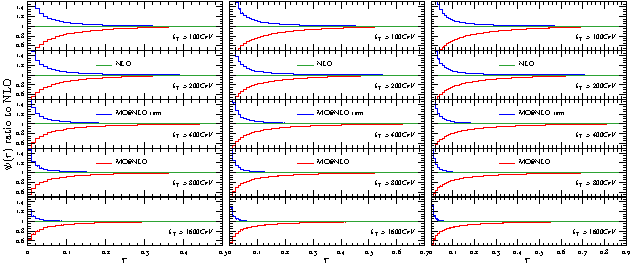
\includegraphics[width=\textwidth]{plots/shapes/hj/hjshapes-crop.pdf}\\
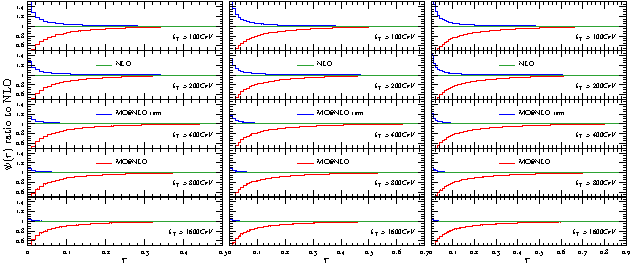
\includegraphics[width=\textwidth]{plots/shapes/zj/zjshapes-crop.pdf}\\
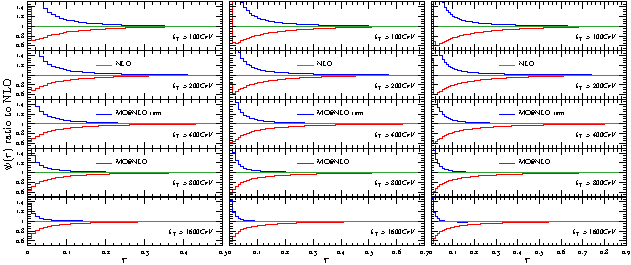
\includegraphics[width=\textwidth]{plots/shapes/jj/jjshapes-crop.pdf}
\caption{Jet shapes for Higgs and Z plus jets and inclusive jets}
\label{fig:jet_shapes_Higgs_Z_jets}
\end{figure}

\section{K-factors}

$\bf JH:$ Note that the nomenclature below may be confusing. I'm happy for other suggestions as to how to display/discuss the figures. 

Figure~\ref{fig:K-factors} top (bottom) shows (left) the transverse momentum spectrum
of the Higgs boson (Z-boson)  as predicted by the fixed-order LO, NLO and NNLO calculation, as well as the
results from a multi-jet merged computation using the 
%\Sherpa 
Sherpa event generator and
the NLO-matched 
%\Herwig 
Herwig result. The NLO, 
%\Sherpa and \Herwig 
Sherpa and Herwig results are all in very good agreement with each other over the range of the plot ($\ge$ 100 GeV). The NNLO normalizations are larger due to the higher order effects included in these calculations. 

Figure~\ref{fig:K-factors} top (bottom) shows (center) shows the $K$-factors (NLO/LO, NNLO/LO, NNLO/NLO, from %\nnlojet) 
nnlojet as a function of the 
Higgs boson (Z boson) $p_T$, for different jet radii; as expected there is no jet size dependence for this
variable.  Also shown (right) are the local K-factors as a function of the lead jet transverse momentum for the two processes, for various jet sizes.  The
$K$-factors for $H+\ge1$ production  are relatively flat as a function of jet $p_T$.  They grow with
increasing jet size, due to inclusion of additional real radiation. The
$K$-factors (NLO/LO and NNLO/LO) for $Z+\ge1$ production  grow rapidly with  jet $p_T$, due to the increasing dominance of dijet production, followed by a Z boson emission. 
The K-factors (NNLO/NLO) are relatively flat, indicating that there are no substantial new subprocesses being added at NNLO. 

\begin{figure}
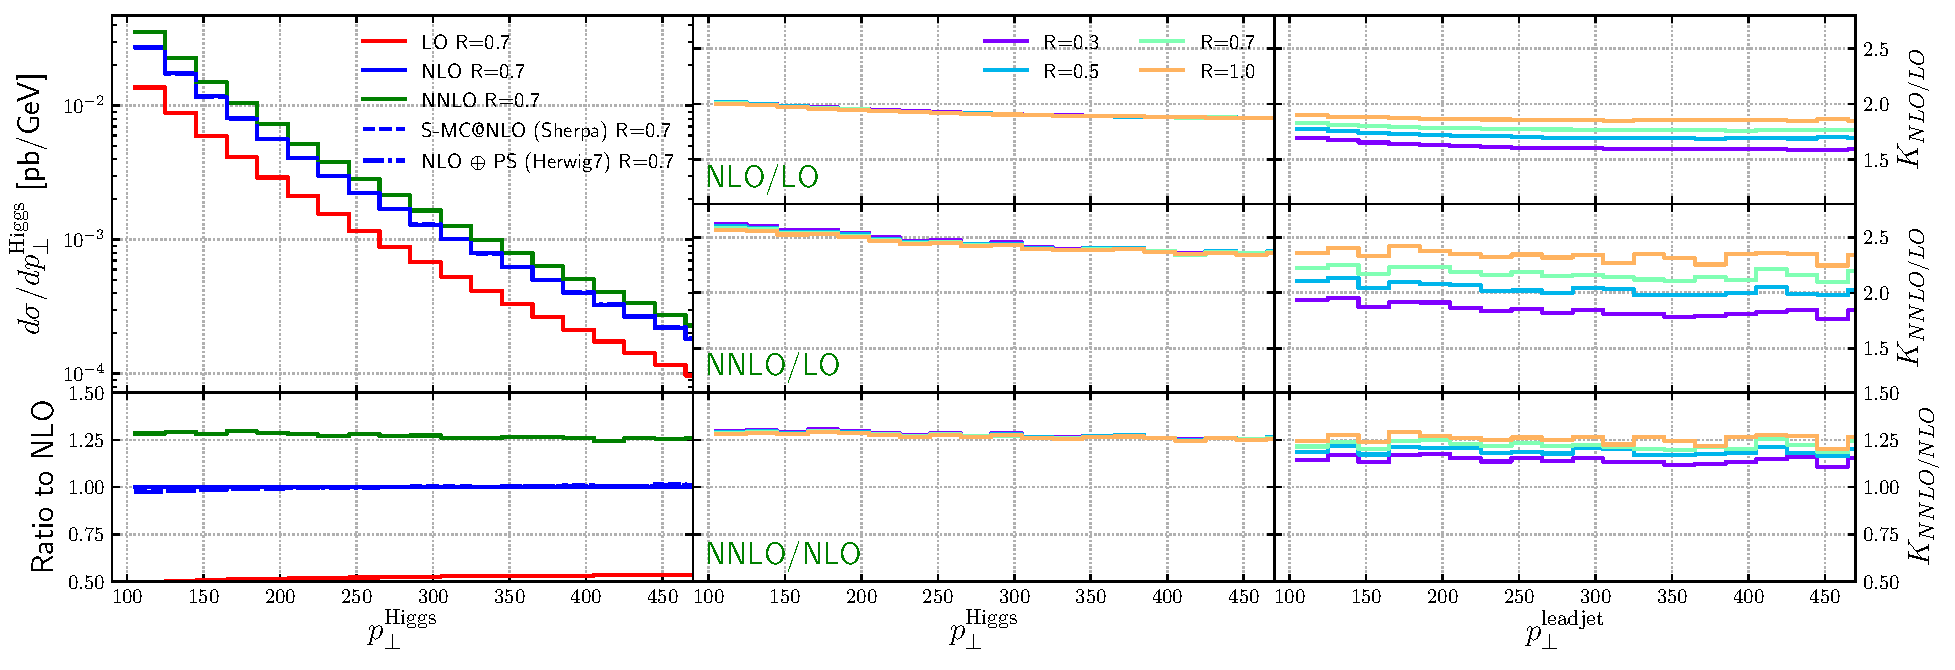
\includegraphics[width=\textwidth]{plots/Fig_V_14_Higgs_2.pdf}
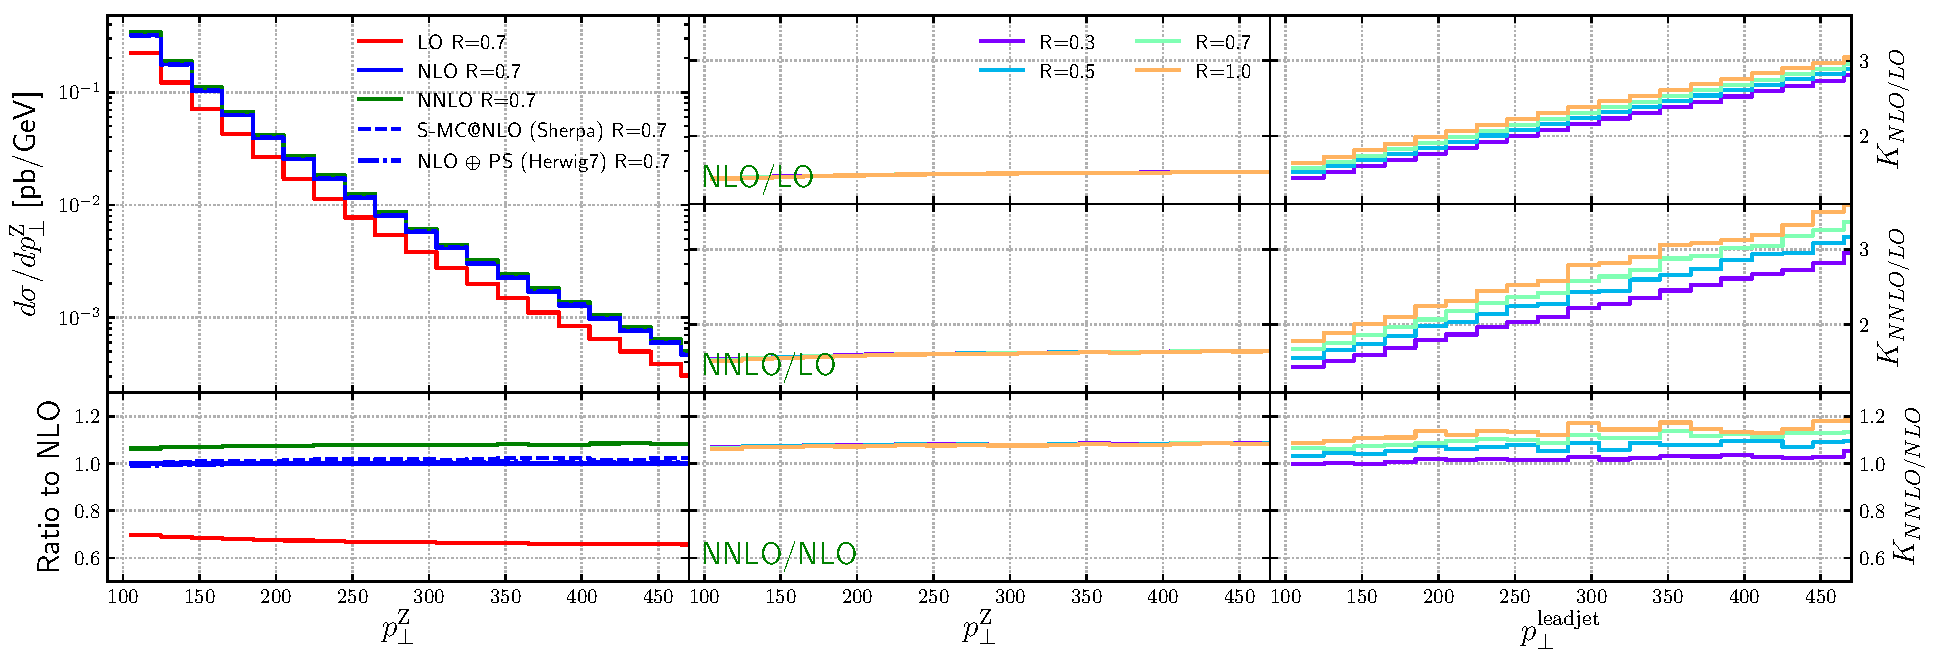
\includegraphics[width=\textwidth]{plots/Fig_V_14_Z_2.pdf}
\caption{K-factors for Higgs and Z plus jets.}
\label{fig:K-factors}
\end{figure}

Figure~\ref{fig:K-factors_jet}(left)  shows the the inclusive jet transverse momentum spectrum  as predicted by the fixed-order LO, NLO and NNLO calculations, for an R-value of 0.7,  as well as the
results from a multi-jet merged computation using the 
%\Sherpa 
Sherpa event generator and
the NLO-matched 
%\Herwig 
Herwig result.

$\bf JH:$ I assume that this is for the inclusive jet pT scale.

In addition, a prediction from 
%\Powheg 
Powheg is included as well. The NLO, 
%\Sherpa, \Herwig and \Powheg 
Sherpa, Herwig and Powheg results are all in very good agreement with each other over the range of the plot ($\ge$ 100 GeV), i.e. there is no significant $\it parton$ $\it shower$ $\it systematic$ and the predictions with parton showers reflect the underlying NLO matrix elements. The NNLO normalizations are larger due to the higher order effects included in these calculations.  $K$-factors (NLO/LO, NNLO/LO, NNLO/NLO, from 
%\nnlojet) 
NNLOJET are shown as a function of jet size,  as a function of the 
inclusive jet  $p_T$, for two different rapidity intervals. Again, the K-factors grow with increasing jet size, as before, and also have a slight slope (NLO/LO, NNLO/LO) as a function of the jet transverse momentum. 

\begin{figure}
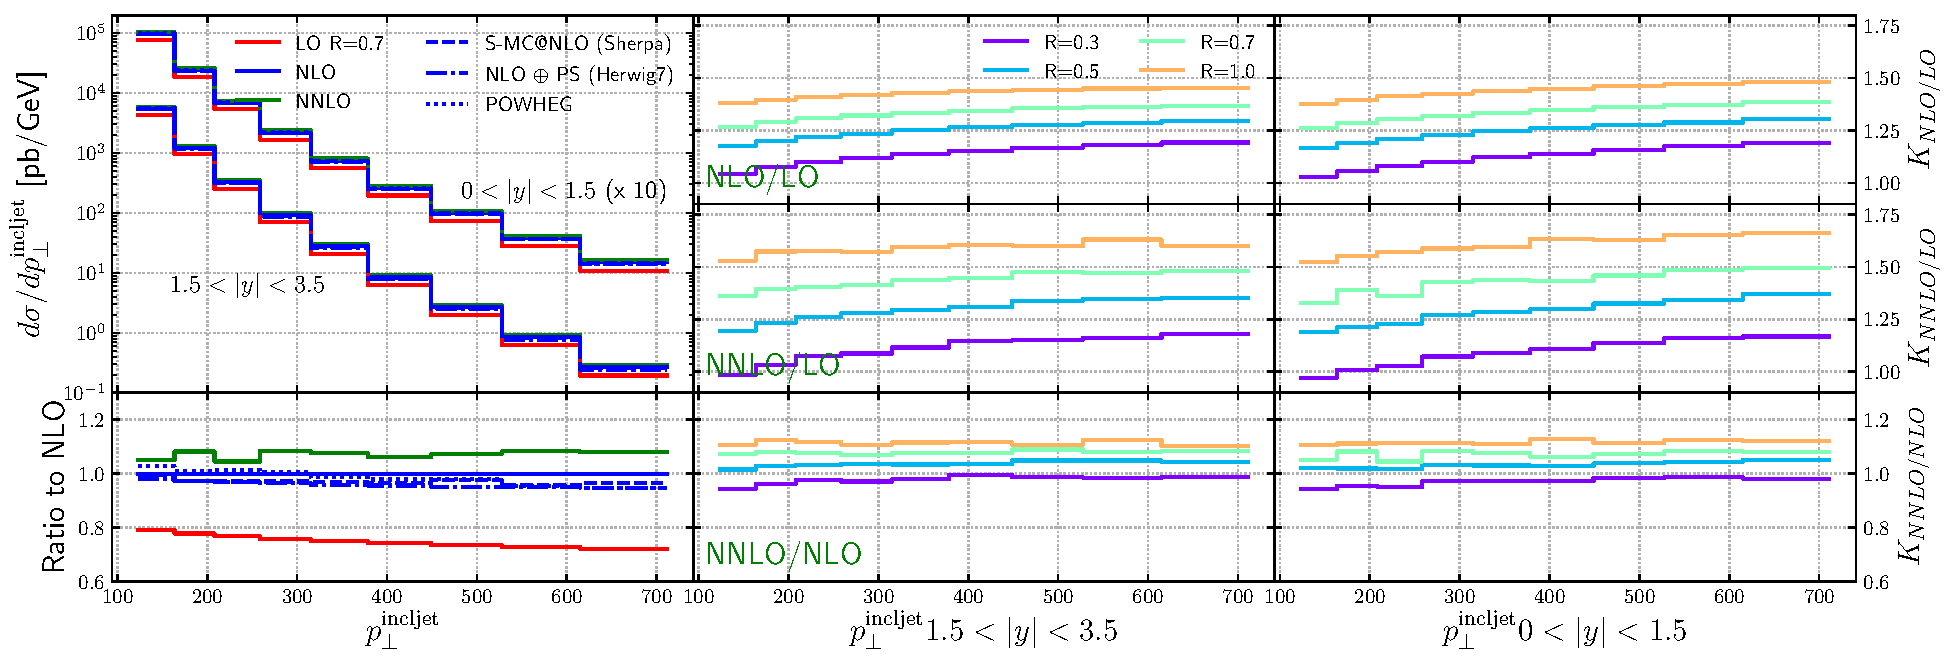
\includegraphics[width=\textwidth]{plots/Fig_V_14_J_2.pdf}
\caption{K-factors inclusive jet production.}
\label{fig:K-factors_jet}
\end{figure}

The cross sections for $H +\ge1$ jet, $Z +\ge1$ jet, and dijet production from 
%\nnlojet 
NNLOJET are shown in Figure~\ref{fig:Comparison_plot}, as a function of the inclusive jet $p_T$ at LO, NLO and NNLO. It is interesting to note that for $H +\ge1$ jet production, the R-dependence is larger at NNLO than at NLO. The R-dependence for $Z +\ge1$ jet production is relatively small both at NLO and NNLO. For dijet production, the R-dependence is relatively large at both NLO and NNLO. 

\begin{figure}
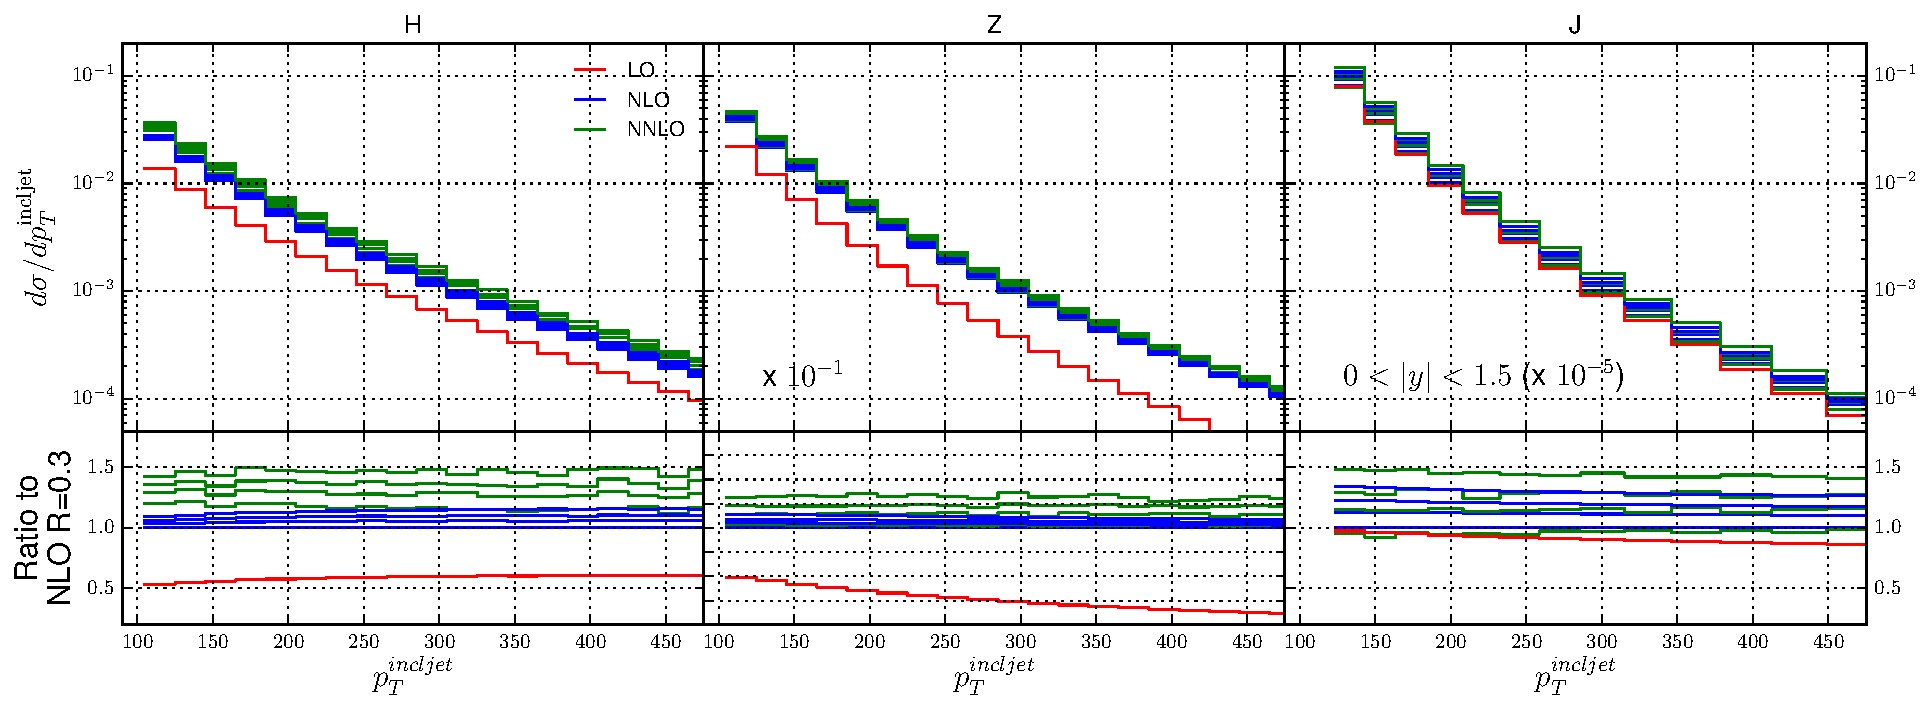
\includegraphics[width=\textwidth]{plots/Comparison_Plot.pdf}
\caption{The cross sections for $H +\ge1$ jet, $Z +\ge1$ jet, and dijet production from 
%\nnlojet
NNLOJET, as a function of the inclusive jet $p_T$ at LO, NLO and NNLO. }
\label{fig:Comparison_plot}
\end{figure}

$\bf JH:$ What conclusions do we draw from these observations? It's mostly gluon jets for Higgs while Z has a fair fraction of quark jets. Why does inclusive jet have a similar behavior at both NLO and NNLO? 



%\begin{figure}
%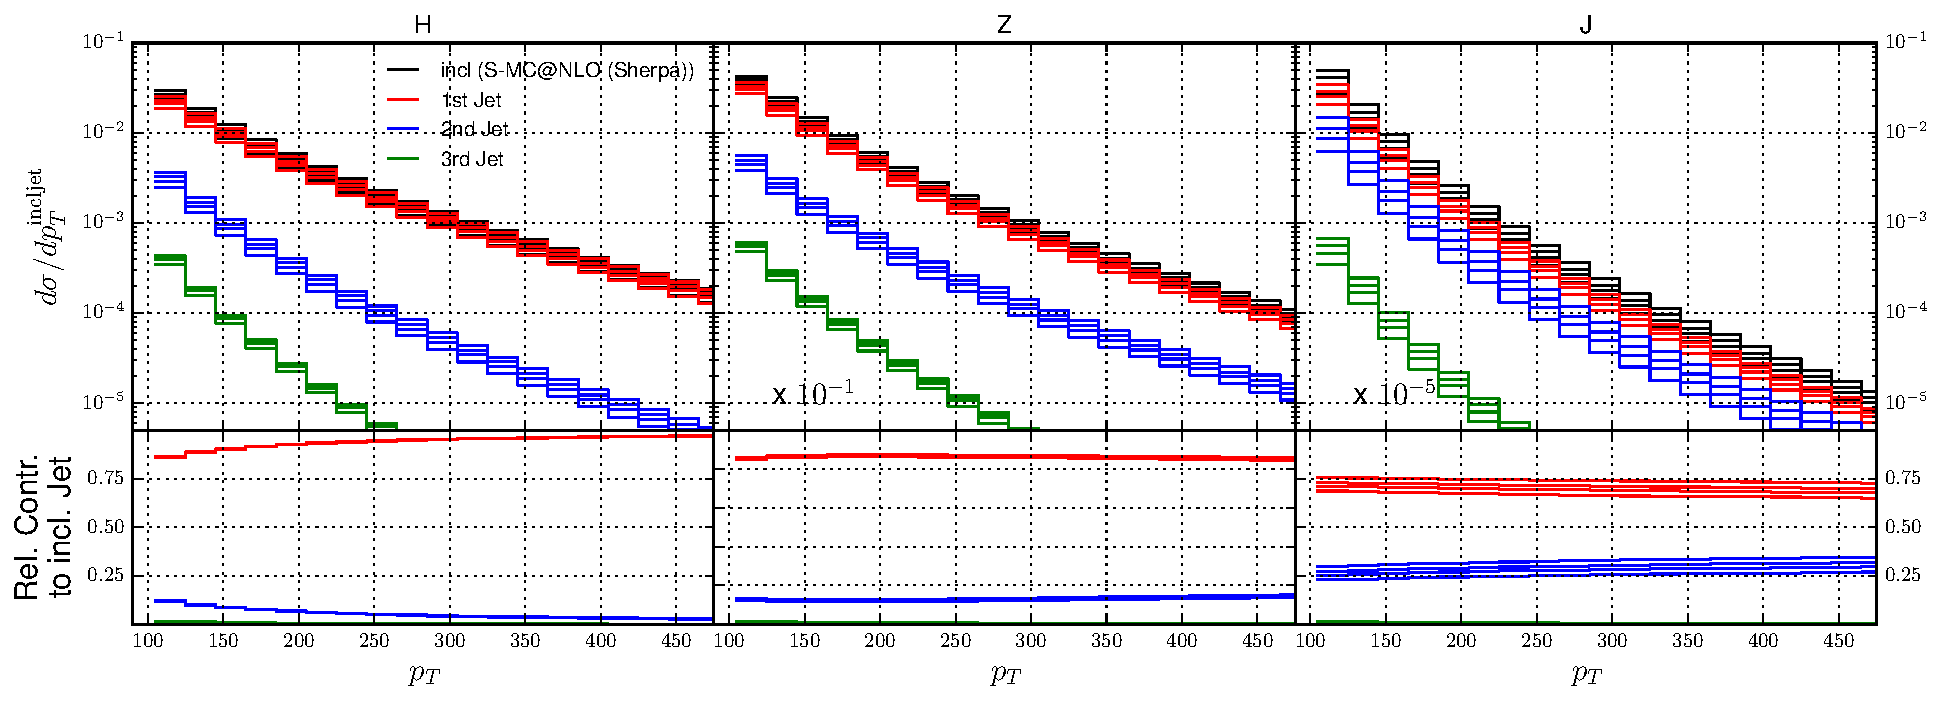
\includegraphics[width=\textwidth]{plots/Comparison_Contributions.pdf}
%\caption{I haven't put in any text yet for the Comparison_Contributions plot. Basically, it just shows that %for H+jet and Z+jet, the dominant jet pT contribution comes from the lead jet, while for dijet production, %both the 1st and 2nd jet strongly contribute.  }
%\label{fig:Comparison_Contributions}
%\end{figure}


\section{Results}

Figure~\ref{fig:SM_Higgs_jet_R:ScaleVariationsFO} shows the cross section scale variations at
LO, NLO and NNLO for $H(Z) +\ge1$ jet production, as a function of the leading jet
transverse momentum, for various jet sizes. The uncertainty bands are given by the
highest and lowest cross section predictions at each order. As expected, the
uncertainties on the cross sections decrease from LO to NLO to NNLO. They also
decrease (slightly) as the jet size decreases, perhaps not surprising given that larger
jet radii lead to inclusion of more real radiative corrections.  

$\bf JH:$ The statement above is from the original paper. I would have expected a larger variation with R of the scale uncertainty. Should we keep that last statement about radiative corrections in? 

The scale uncertainties for $H +\ge1$ jet production are relatively constant as a function of the lead jet transverse momentum. For $Z +\ge1$ jet production, the scale uncertainties increase as the lead jet transverse momentum increases, understandable given the increasing contributions from dijet production as the lead jet tranverse momentum increases. 

Also shown for
comparison are the predictions from the two MEPS calculations (nominally of NLO
accuracy). We scale the MEPS predictions with the $K$-factors derived from the
Higgs(Z) $p_T$ distribution above 150~GeV, see discussion of Fig.~\ref{fig:SM_Higgs_jet_R:KFactorsFO}. For $H +\ge1$ jet production, the two MEPS predictions agree very well with each other and tend to be at the lower end of the scale uncertainty bands for R=0.4, at center of the scale uncertainty bands for R=0.7 and slightly above the center of the scale uncertainty bands for R=1.0. For $Z +\ge1$ jet production, the MEPS predictions again are in agreement with each other, but rapidly increase over the LO results as the lead jet $p_T$ increases (again due to the impact of the dijet contribution, arising only at NLO or above). At NLO, a similar behavior with respect to the NLO scale uncertainty band is observed as was seen for $H +\ge1$ jet. At NNLO, the MEPS predictions are close to the scale uncertainty bands, which are extremely small, especially for R=0.4. 


\begin{figure}[t]
\centerline{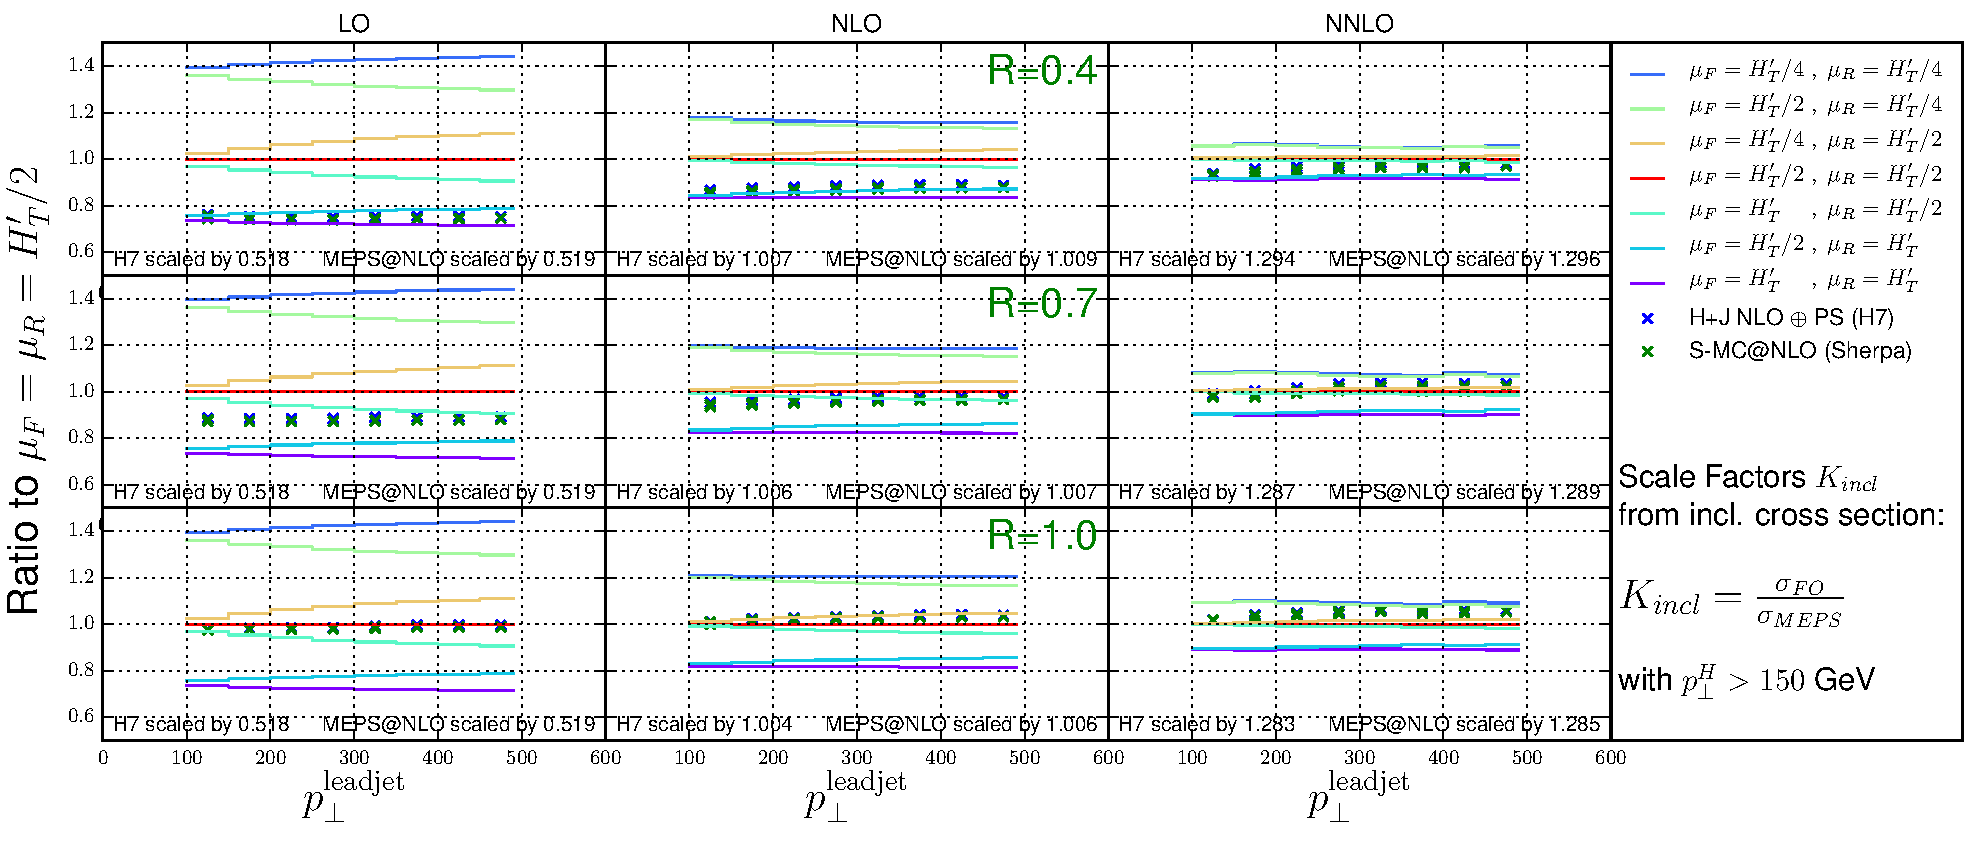
\includegraphics[width=\textwidth]{plots/Fig_V_16_Higgs.pdf}}
\centerline{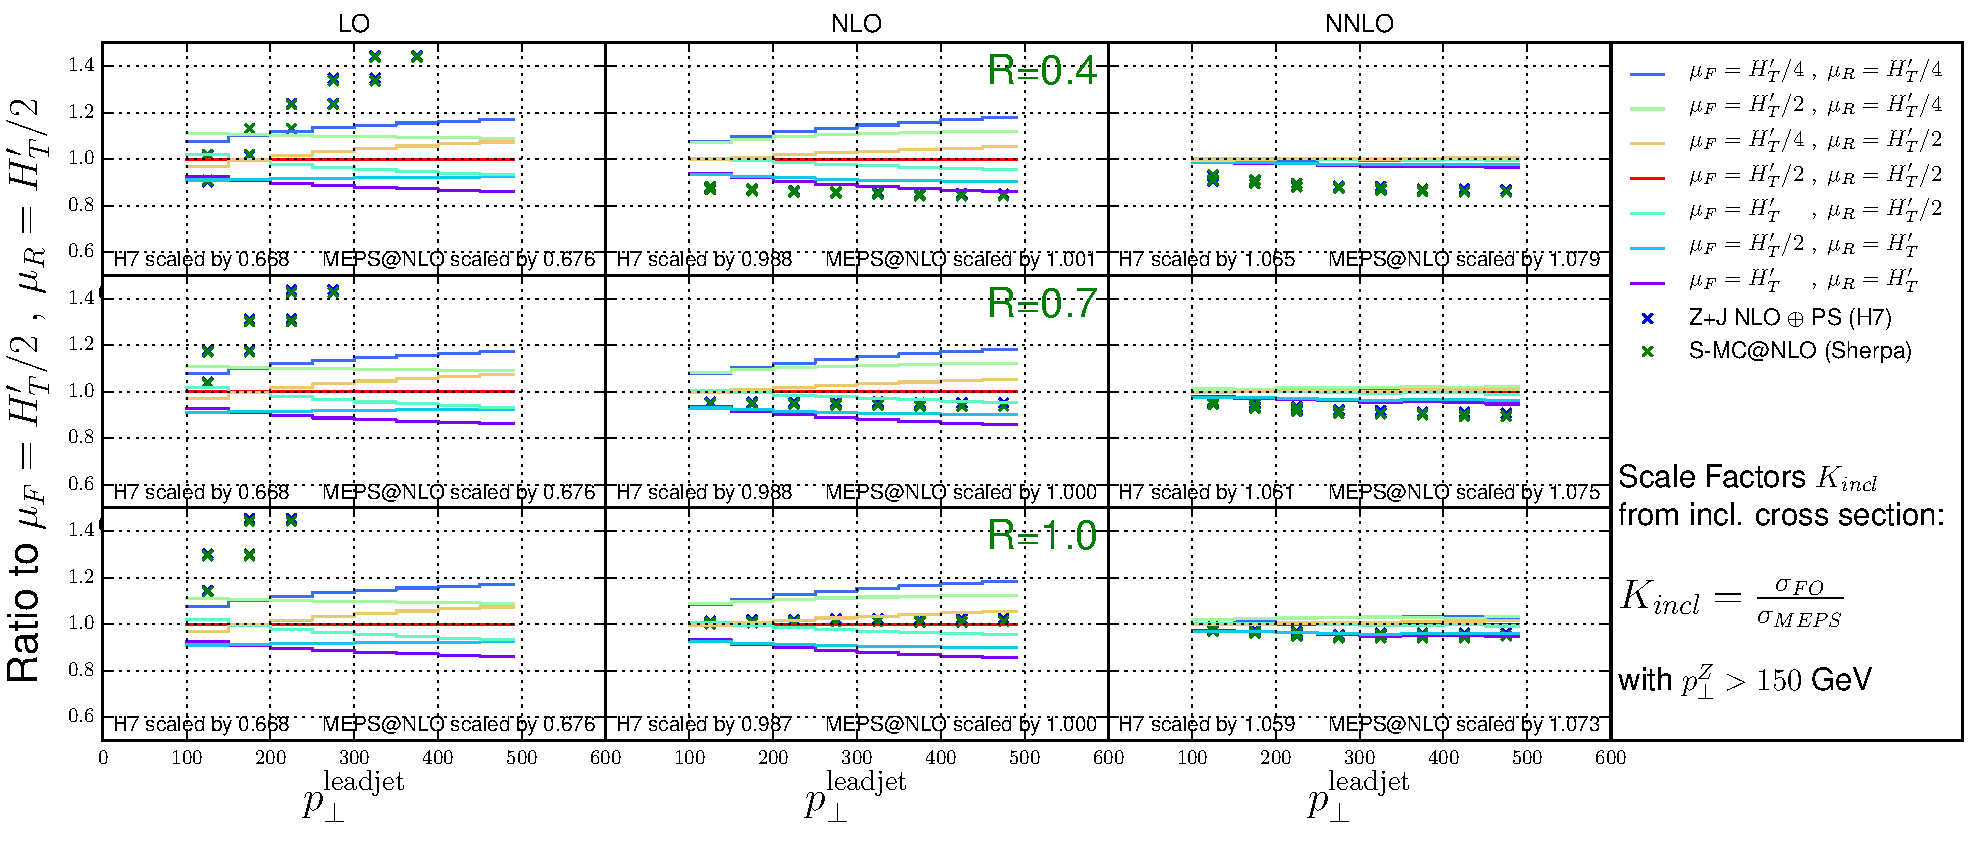
\includegraphics[width=\textwidth]{plots/Fig_V_16_ZJ.pdf}}
\caption{The scale variations at LO, NLO, and NNLO from 
%\nnlojet 
NNLOJET for 3 jet
sizes, as a function of leading jet transverse momentum, are shown.  For comparison,
the nominal NLO MEPS predictions are also shown. The generator predictions are
scaled with the inclusive $K_{incl}$ factor with Higgs(Z) $p_\perp > 150$~GeV,
see Fig.~\ref{fig:SM_Higgs_jet_R:KFactorsFO}. } 
\label{fig:SM_Higgs_jet_R:ScaleVariationsFO}
\end{figure}


$\bf JH:$ In addition to the size of the uncertainty bands as a function of R, should we comment about where the central fit lies inside the uncertainty band? 

Figure~\ref{fig:AccidentalScaleComp_H} shows the leading jet $p_T$ cross sections for $H +\ge1$ jet production for
the different scale choices, at LO, NLO and NNLO, as a function of the jet size $R$.
In this case, a minimum transverse momentum requirement of 150~GeV has been
placed on the leading jet.  We assume this scale to be large enough such that $M_H$
is not the large scale in the process.  The dots for each scale choice have been
fit to a functional form motivated by the expected behavior for jet-vetoed cross
sections.
We assume the leading functional form:
\begin{equation}
f(R)=a+b\log(R)+c\log^2(R) \label{eq:SM_Higgs_jet_R:fit}
\end{equation}
as we expect a logarithmic behaviour for the scales induced by the effective
veto on the cross section by cutting with the jet cone $R$.  The lines in
Fig.~\ref{fig:SM_Higgs_jet_R:AccidentalScaleComp} are then interpolations with 
Eq.~\eqref{eq:SM_Higgs_jet_R:fit} and the fitted values. 
 
Again, the scale variation band is given by the upper and lower curves at each
order. It is notable that the scale uncertainty bands shrink as the jet size
decreases, as mentioned earlier. For very low values of $R$, this improvement in
the uncertainty can be regarded at least partially due to accidental
cancellations that stem from the restrictions in phase space.  Similar effects
were pointed out in the context of exclusive jet rate
measurements~\cite{Stewart:2011cf}. It can also be observed that for each
particular scale, the slope is greater at NNLO than at NLO. The MEPS predictions
are also plotted in the figure, and can be observed to have a greater slope than
even the NNLO predictions.  This can be seen as an effect of either including
(at large $R$) or not excluding (at small $R$) additional semi-hard real emissions,
which have a leading-order scale dependence and therefore induce a large change
in the cross section.

\begin{figure}[t]
  \centerline{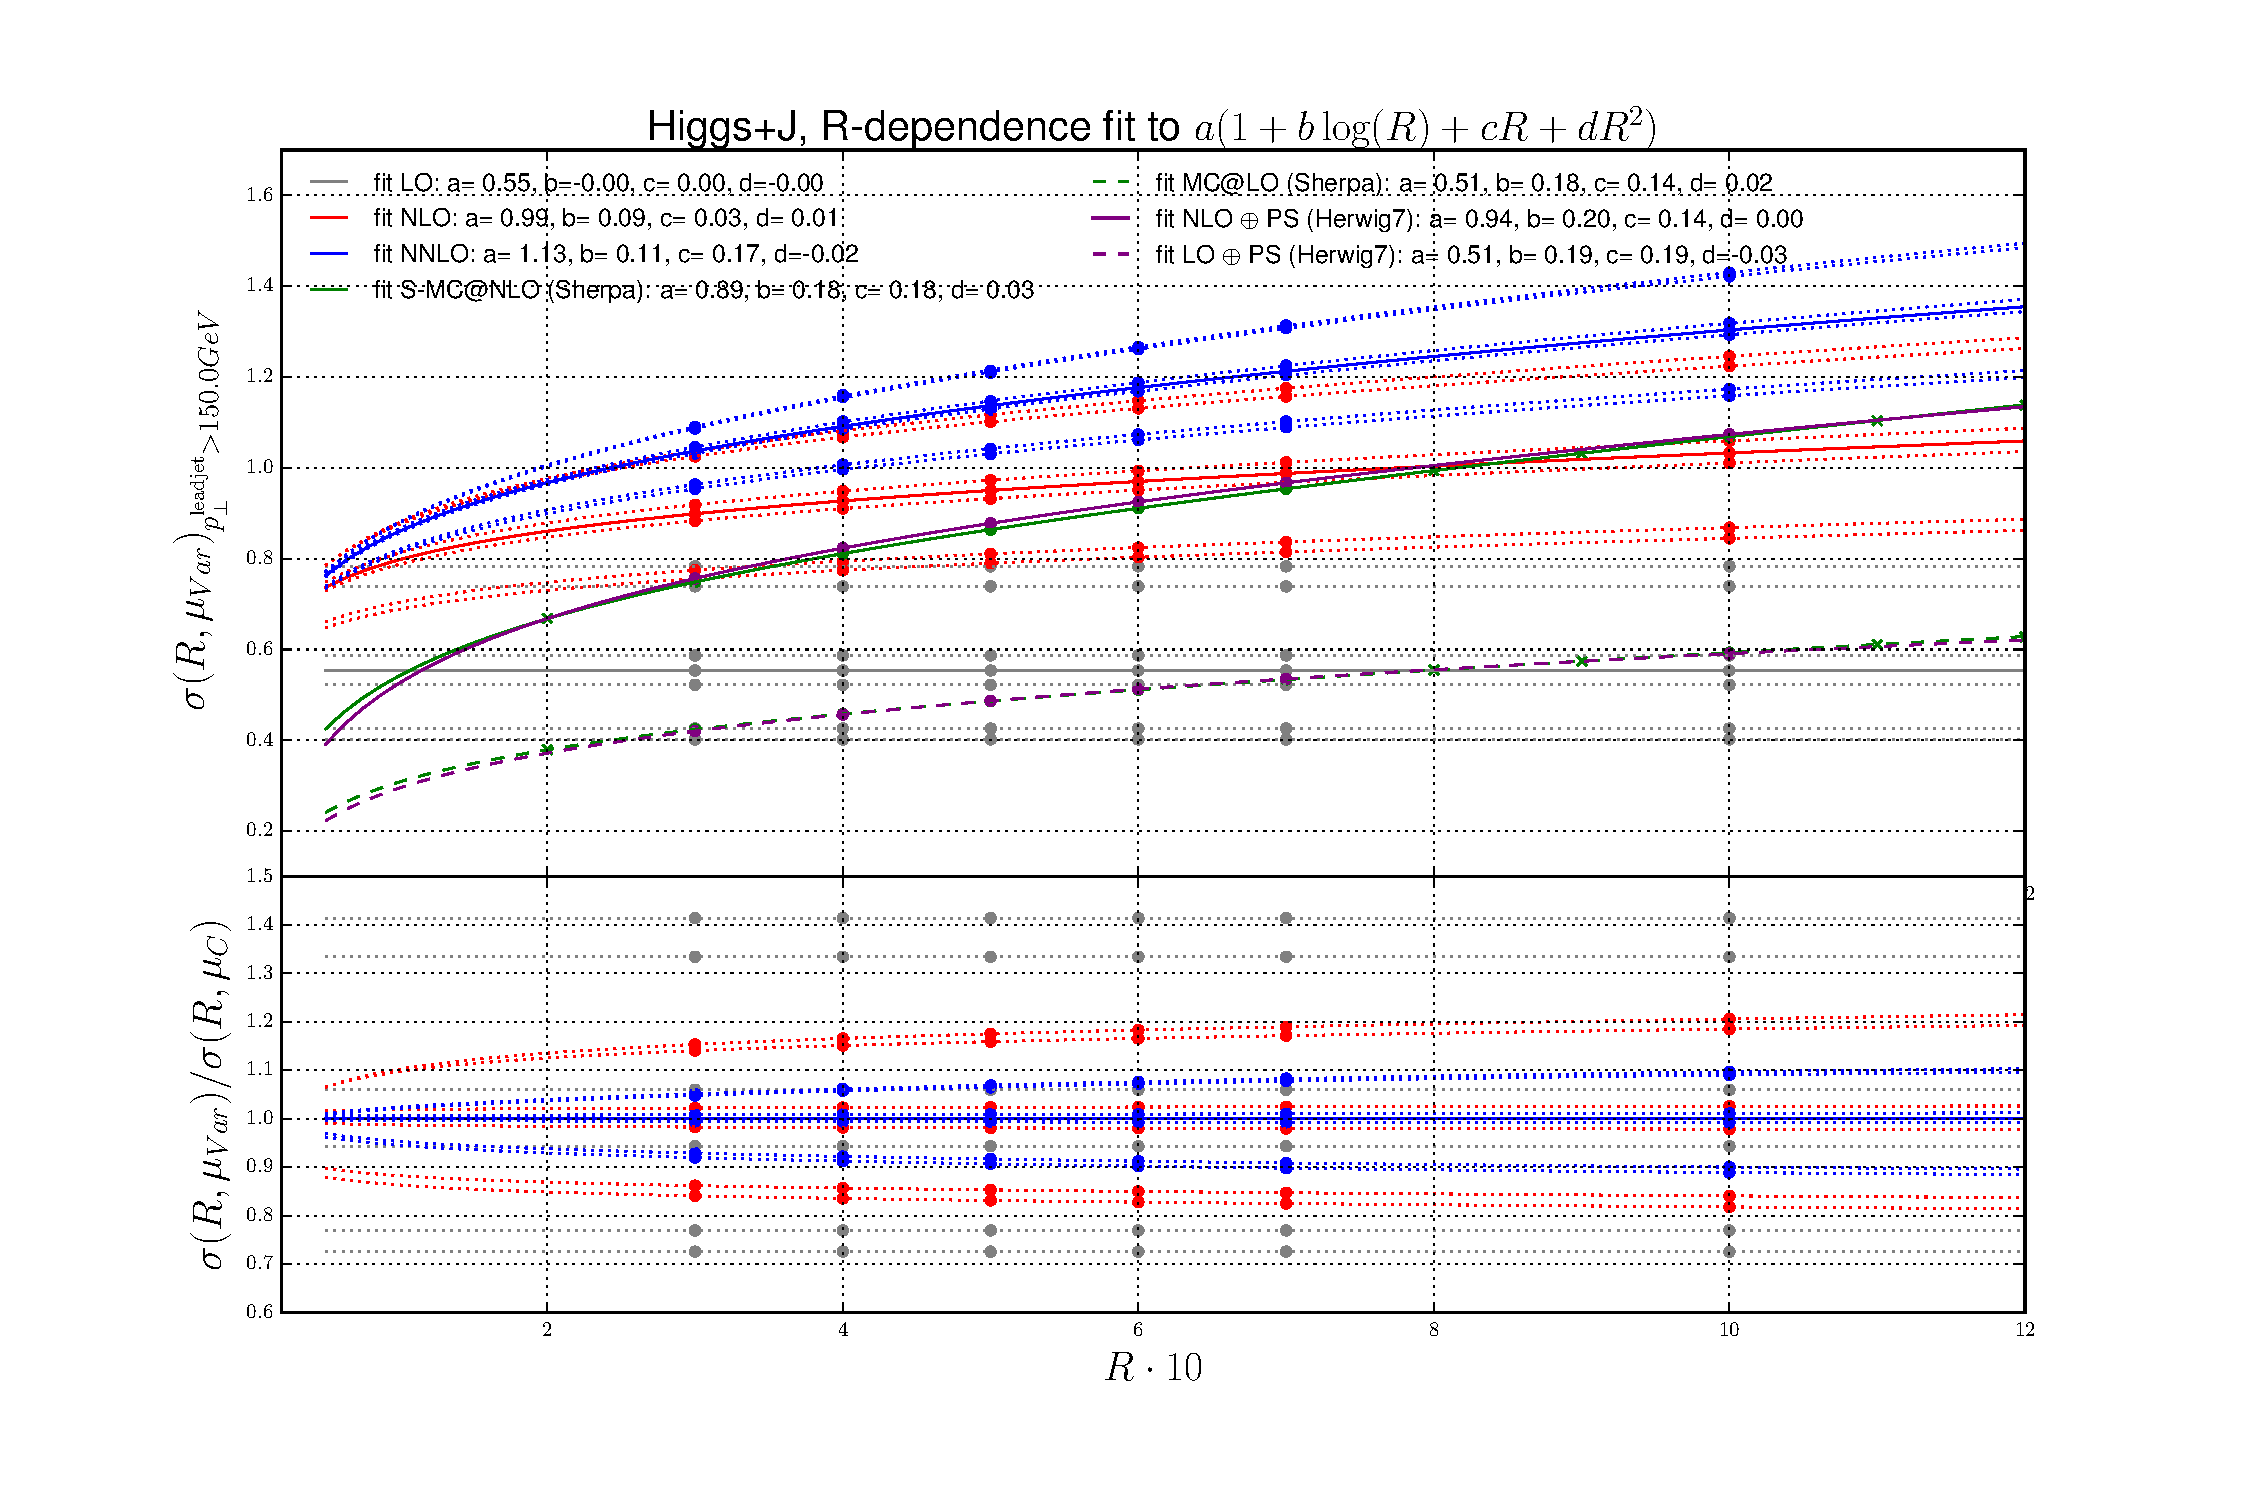
\includegraphics[width=\textwidth]{plots/Fig_V_17_Higgs.pdf}}
  \caption{The $R$-dependence of the cross sections at NLO, NNLO and MEPS are shown, for 
particular scale values, as a function of the jet radius, for $H +\ge1$ jet production, for leading jet transverse momenta above 150~GeV.  
\label{fig:AccidentalScaleComp_H}}
\end{figure}

Figure~\ref{fig:AccidentalScaleComp_Z} shows the leading jet $p_T$ cross sections for $Z +\ge1$ jet production for
the different scale choices, at LO,  NLO and NNLO, as a function of the jet size $R$, and 
again with  a minimum transverse momentum requirement of 150~GeV 
placed on the leading jet. The behavior at NLO is similar to what was observed for Higgs + jet. As for Higgs
+jet, there is a large decrease of the scale uncertainty at NNLO at all $R$ values. In fact, the scale
uncertainty decreases to zero at $R$=0.3, emphasizing the accidental cancellations noted for Higgs+jet. This 
may indicate that the especially small scale uncertainties for $R$=0.4 may be underestimated. 

\begin{figure}[t]
  \centerline{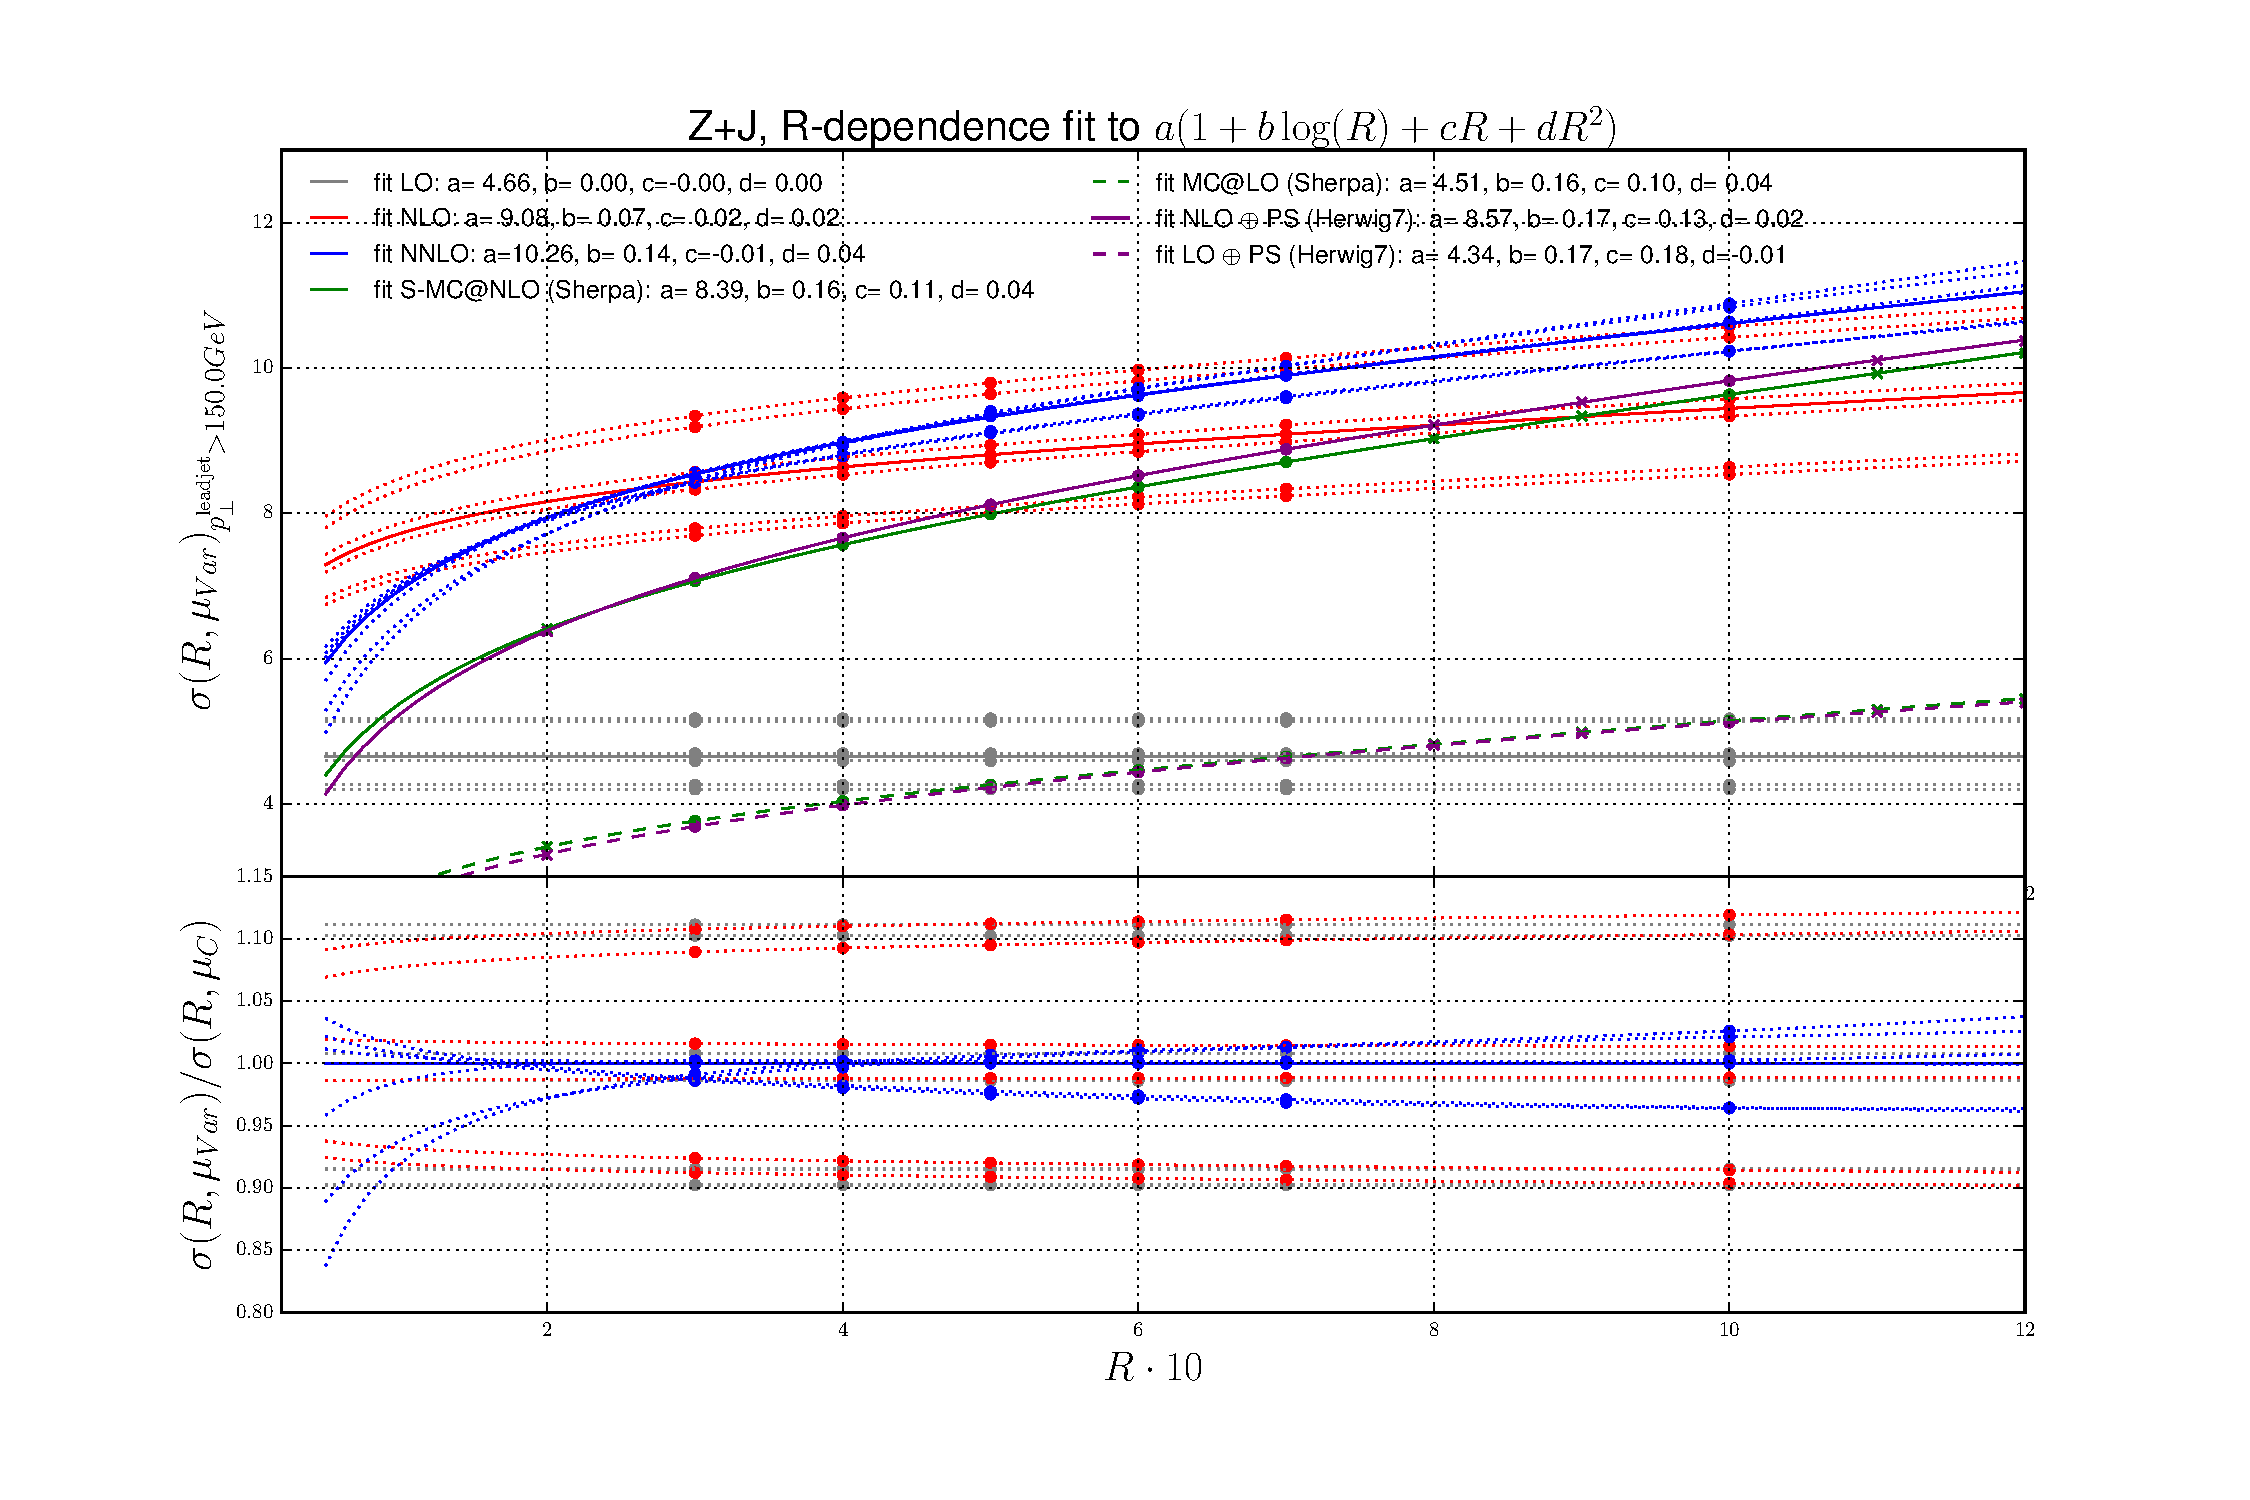
\includegraphics[width=\textwidth]{plots/Fig_V_17_Z.pdf}}
  \caption{The $R$-dependence of the cross sections at NLO, NNLO and MEPS are shown, for 
particular scale values, as a function of the jet radius,for $Z +\ge1$ jet production, for leading jet transverse momenta above 150~GeV.   \label{fig:AccidentalScaleComp_Z}}
\end{figure}

$\bf JH:$ There are scale-dependence plots for 3 possible scales for inclusive jet production. We need to decide how much of a discussion we want to have on this topic. In addition, Joao has some 2-D color plots. 
I have a print-out of the other two scales but can't seem to find the electronic versions. Can whoever has them please upload them? 

Figure~\ref{fig:AccidentalScaleComp_dijet} shows the inclusive jet cross section from dijet production, again at LO, NLO and NNLO, as a function of $R$. Here, the behavior is in some sense more extreme in that the jet $R$ value for zero scale uncertainty is at $R$=0.4, or one of the jet sizes that is commonly used at the LHC. 

\begin{figure}[t]
  \centerline{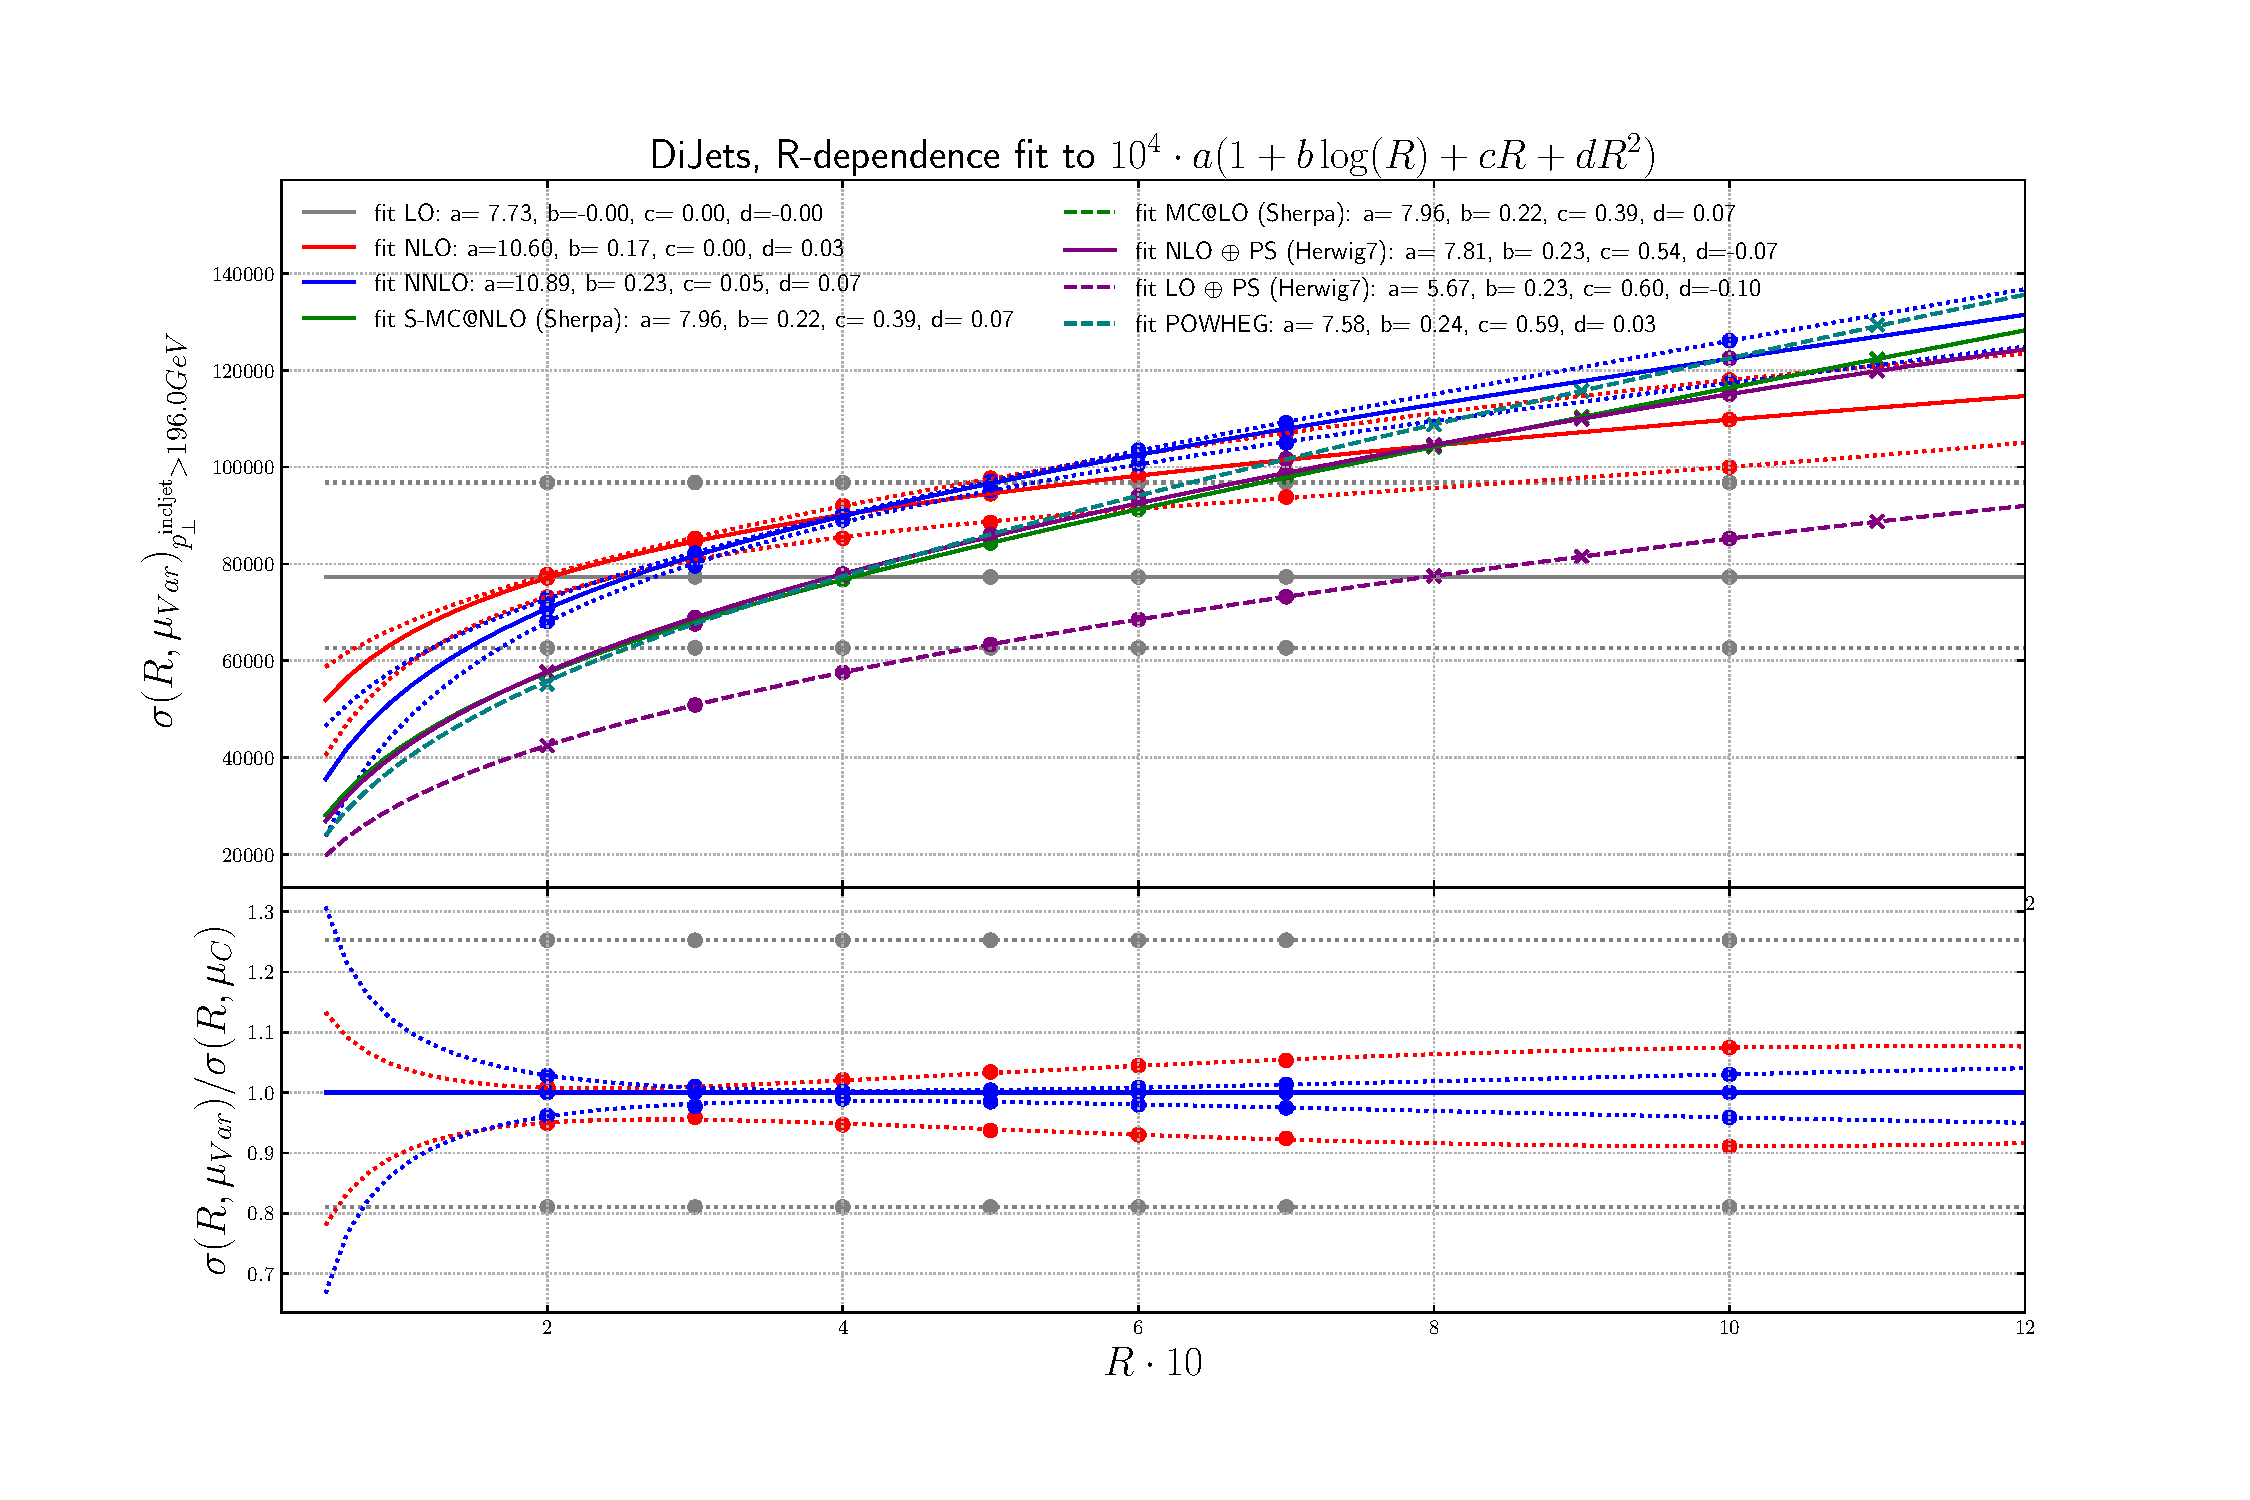
\includegraphics[width=\textwidth]{plots/Fig_V_17_InclJet_1960.pdf}}
  \caption{The $R$-dependence of the cross sections at NLO, NNLO and MEPS are shown, for 
particular scale values, as a function of the jet radius,for dijet production, for leading jet transverse momenta above 150~GeV.   \label{fig:AccidentalScaleComp_dijet}}
\end{figure}

Figure~\ref{fig:SM_Higgs_jet_R:multiratios_vs_NLO_07} shows the cross sections for the Higgs(Z)
transverse momentum  and leading jet transverse momentum  for several
different jet sizes, at LO, NLO and NNLO (from \nnlojet) and from the two MEPS
predictions. All cross sections have been scaled to their respective value for the
reference jet size of $R=0.7$.  At this value we observe the best agreement
between fixed-order and multi-jet merged results, save for an overall
normalization which can be extracted from the Higgs(Z) transverse momentum
spectrum, cf.\ Fig.~\ref{fig:SM_Higgs_jet_R:HiggspTSpectrum}. 

$\bf JH:$ Is this (below) true for Higgs? Not really true for Z. 

The absolute value of the
difference between the fixed-order and the multi-jet merged predictions away
from $R=0.7$ increases roughly proportional to $\log (R/0.7)$
(cf.\ Fig.~\ref{fig:SM_Higgs_jet_R:ps_vs_fo_rpt_higgs}), which is expected due to the
higher-multiplicity real-emission corrections included in the multi-jet merged
calculation. Depending on kinematics they either enhance (at $R>0.7$) or reduce
(at $R<0.7$) the cross section.  

The differences between the MEPS predictions
and those from \nnlojet decrease as the order is raised from NLO to NNLO for both Higgs and Z boson production.  The
difference for Higgs boson production is on the order of 5-10\% for $R=0.4$ at NLO and of the order of less than 5\% at NNLO, relatively flat with $p_T$. For Z boson production, the differences between the MEPS predictions and those from \nnlojet at NLO slightly increase with
increasing $p_T$, and are relatively flat and small at NNLO. 


\begin{figure}[t]
  \centerline{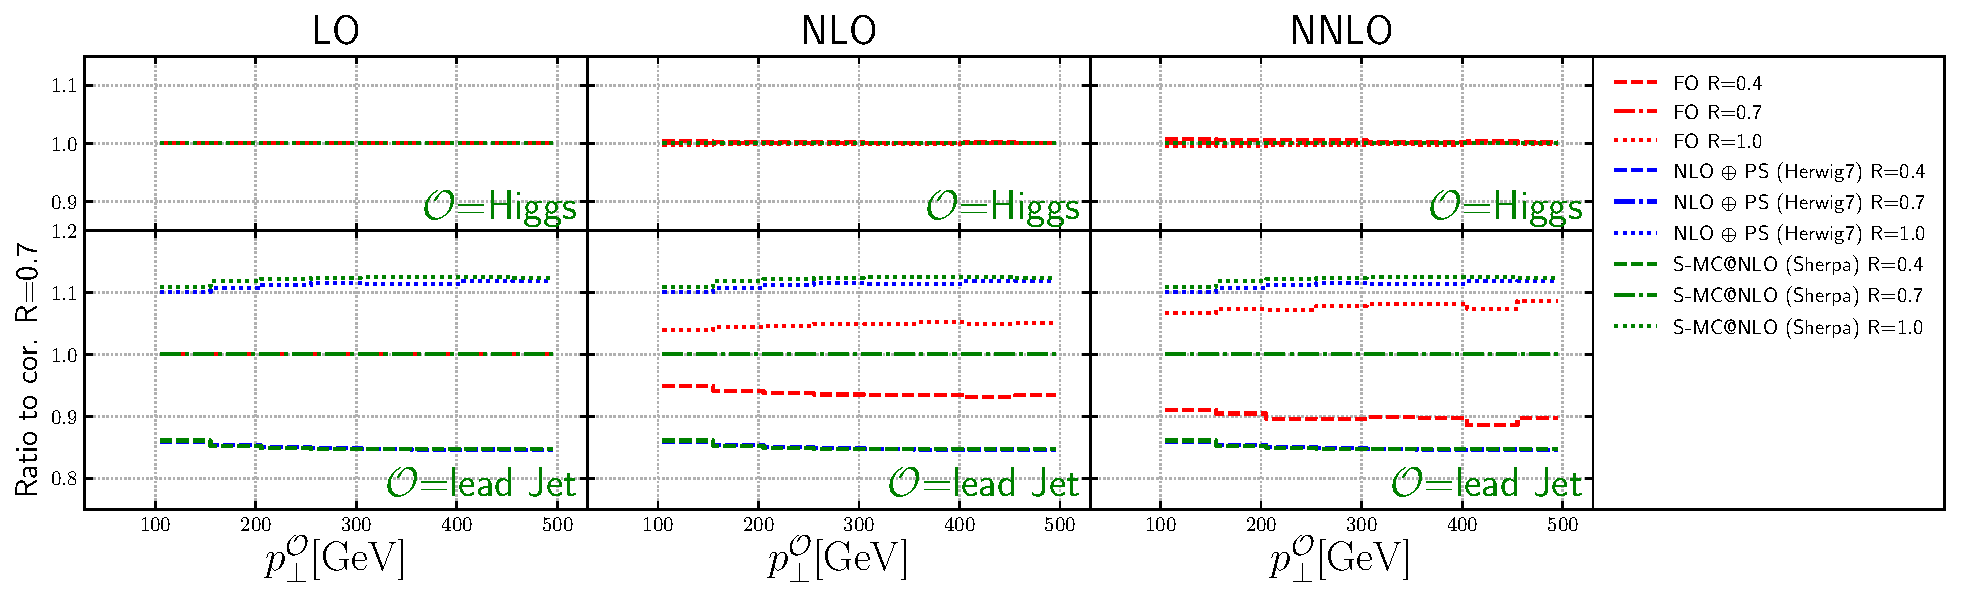
\includegraphics[width=\textwidth]{plots/Fig_V_18_Higgs.pdf}}
  \centerline{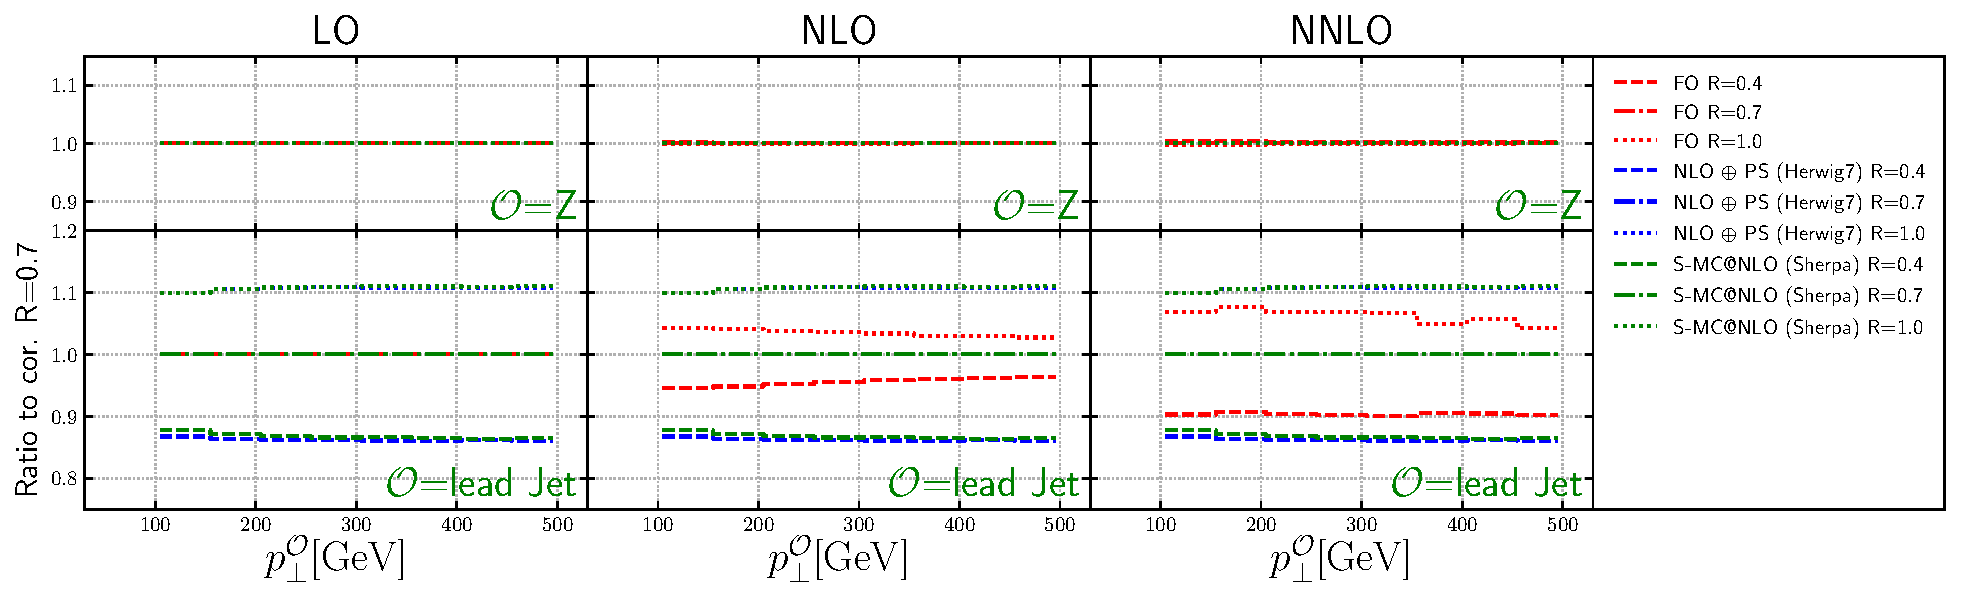
\includegraphics[width=\textwidth]{plots/Fig_V_18_Z.pdf}}
  \caption{The ratio of each cross section (either Higgs(Z) $p_T$ or lead
    jet $p_T$) for specific jet sizes, scaled to the cross section for
    each prediction for a jet size of
    $R=0.7$.  \label{fig:SM_Higgs_jet_R:multiratios_vs_NLO_07}}
\end{figure}

Figure~\ref{fig:SM_Higgs_jet_R:multiratios_vs_NLO_07_jet} shows the cross sections for the inclusive jet $p_T$ distribution for several
different jet sizes, at LO, NLO and NNLO (from \nnlojet) and from the two MEPS
predictions. The ratios to R=0.7 decrease as a function of increasing jet $p_T$ at all orders. 
The differences between the three MEPS predictions and those from \nnlojet are on the order of 10\% at NLO and of the order of 5\% or less at NNLO. 

\begin{figure}[t]
  \centerline{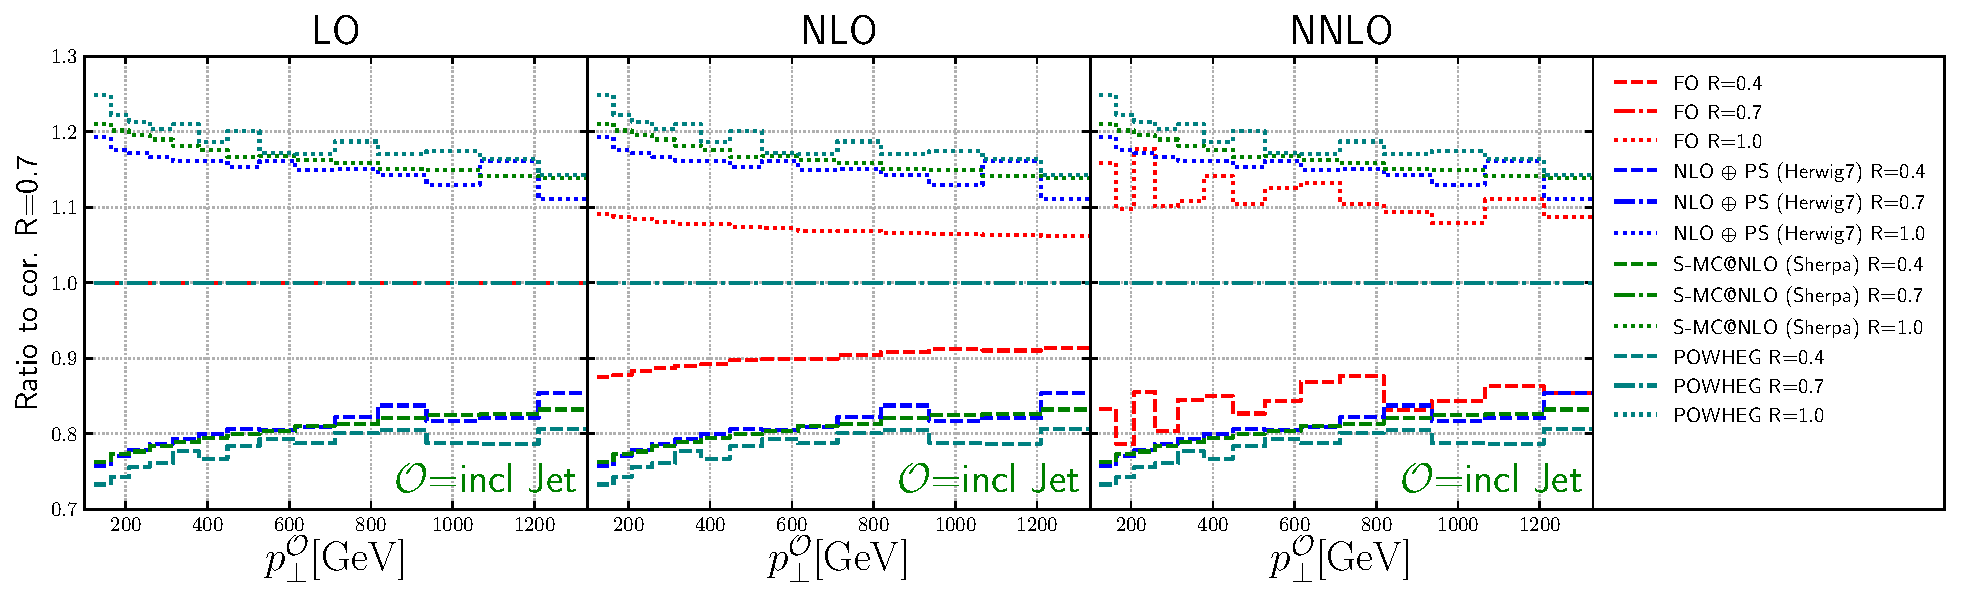
\includegraphics[width=\textwidth]{plots/Fig_V_18_inclJet.pdf}}
  \caption{The ratio of the inclusive jet $p_T$ cross section 
  for specific jet sizes, scaled to the cross section for
    each prediction for a jet size of
    $R=0.7$.  \label{fig:SM_Higgs_jet_R:multiratios_vs_NLO_07_jet}}
\end{figure}

Given the better description of the jet shape provided by the MEPS predictions,
this is an indication of the theoretical uncertainty associated with the
truncation of the perturbative series. The uncertainty is reduced at NNLO as
expected.  It is noteworthy that the ratios in
Fig.~\ref{fig:SM_Higgs_jet_R:multiratios_vs_NLO_07} are relatively flat as a function of the
transverse momenta.%
\footnote{ The flatness may in fact be somewhat accidental as
we are using the EFT and needs to be confirmed upon including finite top mass
effects.}




Figure~\ref{fig:SM_Higgs_jet_R:ps_vs_fo_rpt_higgs} shows the dependence of the relative
difference between a NLO-matched, multi-jet merged prediction from Sherpa and
the NLO fixed-order result as a function of the leading jet transverse momentum
for varying jet radii.  The ratio is flat as a function of the leading jet
$p_T$.  In Fig.~\ref{fig:SM_Higgs_jet_R:AccidentalScaleComp} we compared integrated cross
sections, while here we observe interestingly a similar behaviour for the
differential cross sections.  In the right plot, the projection is with respect
to the radius,  and displays, in grey, the various transverse momentum intervals
and, in coloured, the lowest and highest energies.  Assuming the leading
behaviour is given by Eq.~\eqref{eq:SM_Higgs_jet_R:fit}, and with the flatness in the leading jet
transverse momentum, the linear, (but slightly quadratic) behaviour in the
logarithmic plot is expected.  We note the zero crossing of the curve on the
right-hand side, which corresponds to the best agreement between fixed-order and
matched/merged result, is located at $R \approx$0.7 (see the discussion of
Fig.~\ref{fig:SM_Higgs_jet_R:multiratios_vs_NLO_07}). In configurations where the jet rapidity
is zero, this corresponds to a roughly equal partitioning of the rapidity
phase-space into collinear sectors for color dipoles spanned between the
initial-state partons and the final-state jet. 

\begin{figure}[t]
  \centerline{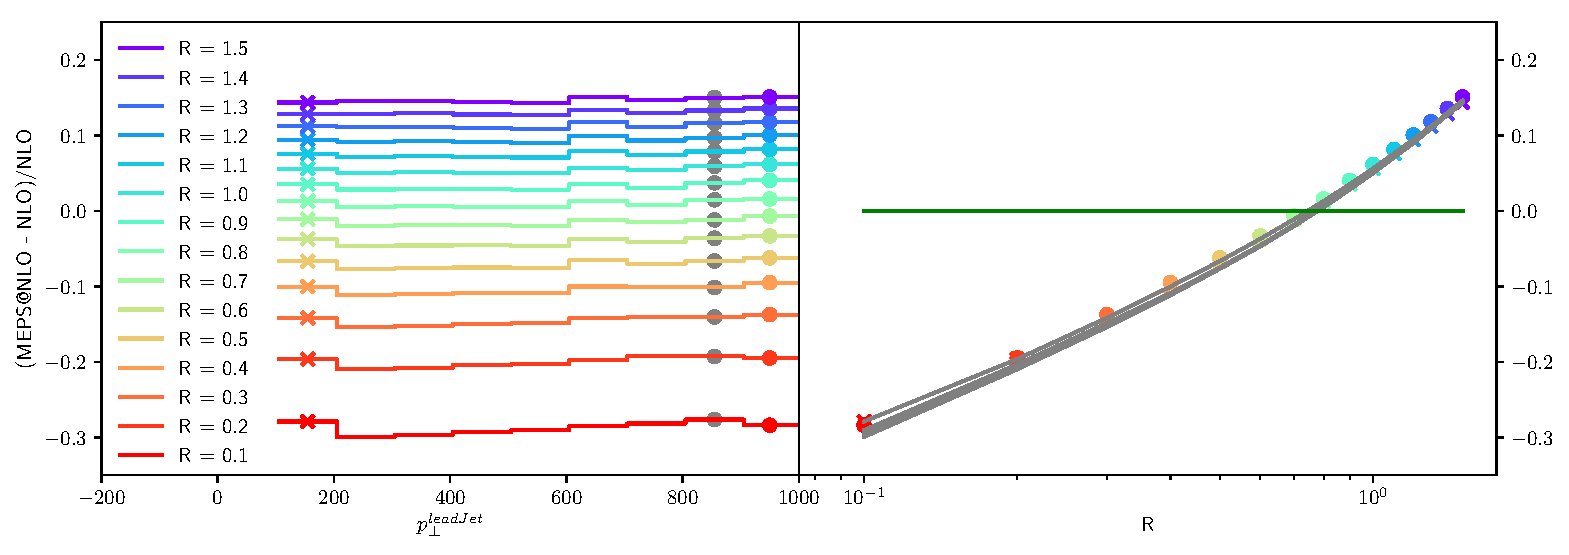
\includegraphics[width=\textwidth]{plots/zhjets_Fig8}}
  \caption{Relative difference between the NLO-matched and multi-jet merged
    prediction to the fixed-order result as a function of the leading jet transverse
    momentum and the jet radius.\label{fig:SM_Higgs_jet_R:ps_vs_fo_rpt_higgs}}
\end{figure}

$\bf JH:$ We need the similar plots for Z+jets and for dijets. 

Finally, for comparison, in Fig.~\ref{fig:SM_Higgs_jet_R:ratio}, we show a (simplified) plot
of the comparison of predictions carried out in Les Houches
2015~\cite{Badger:2016bpw} for the leading jet transverse momentum.  For these
particular scale choices, the NNLO~\cite{Boughezal:2015aha} and
NLO~\cite{vanDeurzen:2013rv,Cullen:2013saa,Greiner:2015jha} give essentially the
same result. The predictions from Sherpa and Herwig agree with NNLO at low
$p_T$, but fall 10-15\% below at higher $p_T$.  This can be due partially to
differences in the scale choices between each prediction in the figure,
differences between the scale choices used in~\cite{Badger:2016bpw} compared to
ours, and to the jet shape differences explored in detail in this note.


\begin{figure}[t]
  \centerline{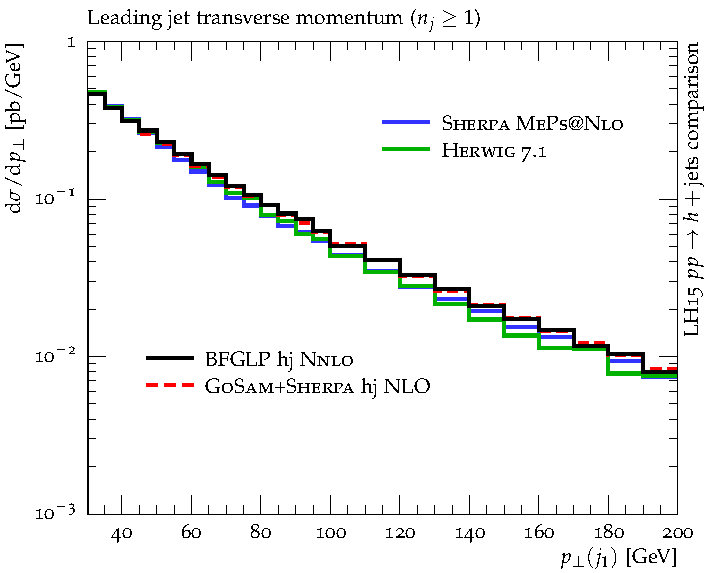
\includegraphics[width=0.48\textwidth]{plots/zhjets_main.pdf}\hfill
    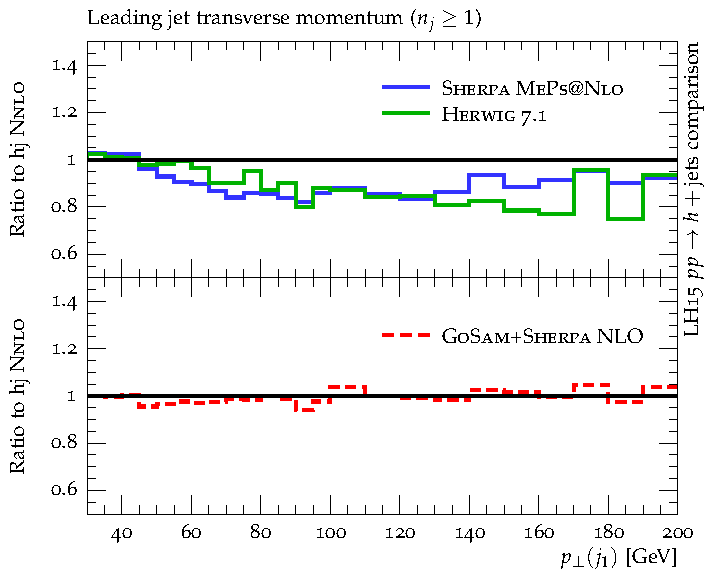
\includegraphics[width=0.48\textwidth]{plots/zhjets_ratio.pdf}}
%  \centerline{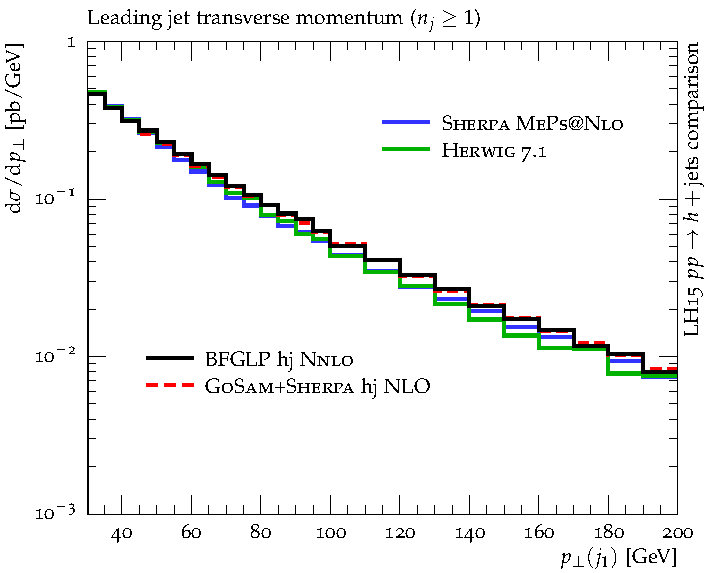
\includegraphics[scale=0.5]{plots/zhjets_main.pdf}
%    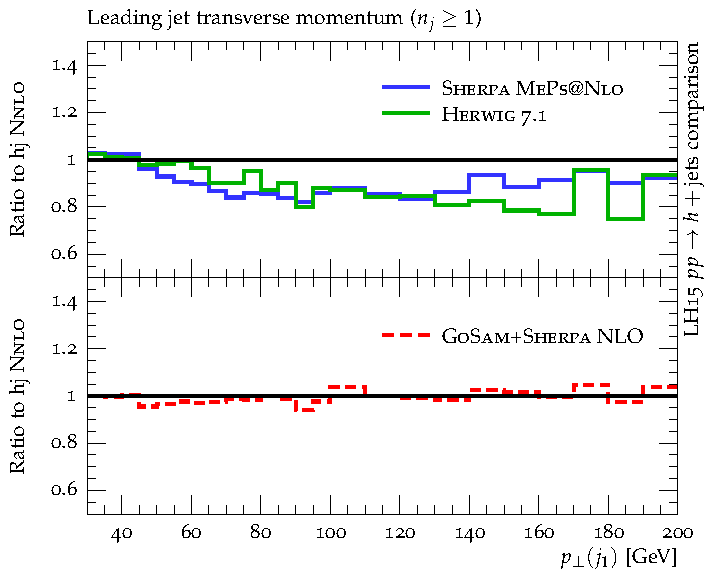
\includegraphics[scale=0.5]{plots/zhjets_ratio.pdf}}
%    \includegraphics[scale=0.5]{plots/ratio.pdf}}
  \caption{Predictions for the leading jet transverse momentum cross sections, for NLO, 
    NNLO and MEPS calculations, from the 2015 Les Houches study~\cite{Badger:2016bpw}.\label{fig:SM_Higgs_jet_R:ratio}}
\end{figure}


\subsection{Outlook}
Searches for new physics, as well as a better understanding of standard model
physics, require an increasing level of precision, both for measurement and for
theory. For differential distributions for $H+\ge1$ jet, the highest level of
precision is obtained with NNLO predictions. Matched NLO plus parton shower
predictions (MEPS) provide a more complete event description, but at a level of
precision one order of $\alpha_s$ lower (although with a more complete
logarithmic treatment).  Most physics measurements at the LHC make use of
relatively small jet sizes (anti-$k_T$ with $R=0.4$), and $H(Z)+\ge1$ jet production and dijet
production are no
exception.  There can be differences between fixed order and MEPS predictions
for the same observable just due to the different estimates of the amount of jet
energy contained in a jet of radius $R$. These differences can be comparable to
the size of the scale uncertainty for the cross section at that order. 

In this contribution, we have reported on an investigation of the impact of
different jet sizes on Higgs (Z)  boson plus jet, and dijet, physics at the LHC, paying close
attention to the impact of the jet size on $K$-factors, on scale uncertainties,
and on differences between fixed order and MEPS predictions. Better
understanding of the issues described in this contribution may allow an
improvement in the accuracy, and precision,  of such predictions at the LHC.

\subsection{Les Houches Manifesto}

We expect ME+PS predictions to differ from the underlying ME predictions in regions where (1) there is a large sensitivity to jet shapes (typically small R jets), (2) there is a restriction in phase space such that soft gluon resummation effects are important, (3) the observable contains multiple, disparate  scales, (4) the observable depends on a higher multiplicity final state than can be produced by the matrix element. Such differences should be smaller at NNLO than at NLO. The corollary would be that, except for (4), the other effects result in 
potentially large logs. Large parton shower effects in the absence of such large logs should be viewed with suspicion, as should large differences between parton shower predictions in general. Thus, it is useful to compare ME+PS predictions with their underlying fixed order backbone. 

JB: We further expect the ME+PS and ME predictions differ from full simulations when multiple parton interactions (MPI) (small $p_T$ and/or large R) or hadronisation  (small $p_T$ and/or small R) effects become important. 
JH: The issue isn't whether there are differences, but whether those corrections can be factorized from ME+PS to ME. 


\bibliography{journal.bib}

\end{document}
